% Generated fragments require trusted human review before compilation.
% This binder never requests shell escape or runs external tools.
\documentclass[11pt]{article}
% Trusted shared apparatus. Requires LuaLaTeX; never use shell escape.
\usepackage{fontspec}
\defaultfontfeatures{Ligatures=TeX}
\IfFontExistsTF{Noto Serif}{\setmainfont{Noto Serif}}{%
  \IfFontExistsTF{DejaVu Serif}{\setmainfont{DejaVu Serif}}{%
    \IfFontExistsTF{Times New Roman}{\setmainfont{Times New Roman}}{%
      \PackageError{gelfand-binder}{No configured Cyrillic serif font installed}{Install Noto Serif or DejaVu Serif, or select an installed Cyrillic font.}%
    }%
  }%
}
\IfFontExistsTF{Noto Sans}{\setsansfont{Noto Sans}}{%
  \IfFontExistsTF{DejaVu Sans}{\setsansfont{DejaVu Sans}}{\setsansfont{Arial}}%
}
\IfFontExistsTF{Noto Sans Mono}{\setmonofont{Noto Sans Mono}}{%
  \IfFontExistsTF{DejaVu Sans Mono}{\setmonofont{DejaVu Sans Mono}}{\setmonofont{Courier New}}%
}
\usepackage[a4paper,margin=22mm]{geometry}
\usepackage{amsmath,amssymb,amsthm,mathtools}
\usepackage{xcolor}
\usepackage{tikz}
\usepackage{tikz-cd}
\usetikzlibrary{arrows.meta,positioning,calc}
\usepackage{hyperref}
\hypersetup{unicode=true,colorlinks=true,linkcolor=blue,pdftitle={Gelfand transcription binder}}
\newtheorem{theorem}{Theorem}
\newtheorem{lemma}{Lemma}
\newtheorem{proposition}{Proposition}
\newtheorem{corollary}{Corollary}
\theoremstyle{definition}
\newtheorem{definition}{Definition}
\newtheorem{example}{Example}
\theoremstyle{remark}
\newtheorem{remark}{Remark}
\setlength{\parindent}{0pt}
\setlength{\parskip}{0.55em}
\setlength{\emergencystretch}{3em}
\newcommand{\SourcePage}[2]{%
  \clearpage\phantomsection\label{#1:source-page}%
  \addcontentsline{toc}{subsection}{#1}%
  {\small\sffamily\color{blue!60!black}Source scan frame: #1; visible page/leaf label: #2}\par\medskip%
}
\newcommand{\Unclear}[3]{%
  \begingroup\color{orange!70!black}%
  [Unresolved reading #1/#2: #3]\endgroup%
}
\newcommand{\Incomplete}[3]{%
  \par\begingroup\color{red!65!black}\textbf{Incomplete #1/#2:} #3\endgroup\par%
}
\newcommand{\SourceFigure}[3]{%
  \par\begingroup\color{blue!60!black}\textbf{\hyperref[#1:source-page]{Source figure #1/#2}:} #3%
  \par\textit{Consult the authoritative scan at this locator.}\endgroup\par%
}



% Reader layout only. Original diplomatic text is retained verbatim.
\setlength{\parskip}{0.35em}
\setlength{\emergencystretch}{4em}
\renewcommand{\SourcePage}[2]{%
  \par\addvspace{1em}\phantomsection\label{#1:source-page}%
  \addcontentsline{toc}{subsection}{#1}%
  {\footnotesize\sffamily\color{blue!55!black}#1%
    \def\givenlabel{#2}\def\nolabel{unlabelled}%
    \ifx\givenlabel\nolabel\else\quad[номер в источнике: #2]\fi
  }\par\nobreak\smallskip%
}
\renewcommand{\Unclear}[3]{%
  \begingroup\color{orange!65!black}%
  \ifmmode\text{[неясно: #3]}\else[неясно: #3]\fi\endgroup%
}
\renewcommand{\Incomplete}[3]{%
  \par\begingroup\color{red!60!black}\textbf{Неразобранный фрагмент:} #3%
  \endgroup\par%
}
\renewcommand{\SourceFigure}[3]{%
  \par\begingroup\color{blue!55!black}\textbf{Рисунок:} #3%
  \par{\small\textit{Исходный рисунок: \hyperref[#1:source-page]{#1}, #2.}}%
  \endgroup\par%
}
\hypersetup{pdftitle={Семинар И. М. Гельфанда. Дипломатическая транскрипция},pdfauthor={},pdfsubject={Русское рабочее издание с отмеченными сомнительными чтениями}}

\usepackage[normalem]{ulem}
\usepackage{newunicodechar}
\usepackage{adjustbox}
\newfontfamily\SourceSymbolFont{Segoe UI Symbol}
\newfontfamily\SourceCJKFont{MS Gothic}
\let\DiplomaticMathUnderline\underline
\renewcommand{\underline}[1]{\ifmmode\DiplomaticMathUnderline{#1}\else\uline{#1}\fi}
\newunicodechar{→}{\ifmmode\text{{\SourceSymbolFont\char"2192}}\else{\SourceSymbolFont\char"2192}\fi}
\newunicodechar{⇒}{\ifmmode\text{{\SourceSymbolFont\char"21D2}}\else{\SourceSymbolFont\char"21D2}\fi}
\newunicodechar{∀}{\ifmmode\text{{\SourceSymbolFont\char"2200}}\else{\SourceSymbolFont\char"2200}\fi}
\newunicodechar{∂}{\ifmmode\text{{\SourceSymbolFont\char"2202}}\else{\SourceSymbolFont\char"2202}\fi}
\newunicodechar{∈}{\ifmmode\text{{\SourceSymbolFont\char"2208}}\else{\SourceSymbolFont\char"2208}\fi}
\newunicodechar{∌}{\ifmmode\text{{\SourceSymbolFont\char"220C}}\else{\SourceSymbolFont\char"220C}\fi}
\newunicodechar{√}{\ifmmode\text{{\SourceSymbolFont\char"221A}}\else{\SourceSymbolFont\char"221A}\fi}
\newunicodechar{∞}{\ifmmode\text{{\SourceSymbolFont\char"221E}}\else{\SourceSymbolFont\char"221E}\fi}
\newunicodechar{∧}{\ifmmode\text{{\SourceSymbolFont\char"2227}}\else{\SourceSymbolFont\char"2227}\fi}
\newunicodechar{∩}{\ifmmode\text{{\SourceSymbolFont\char"2229}}\else{\SourceSymbolFont\char"2229}\fi}
\newunicodechar{∪}{\ifmmode\text{{\SourceSymbolFont\char"222A}}\else{\SourceSymbolFont\char"222A}\fi}
\newunicodechar{∫}{\ifmmode\text{{\SourceSymbolFont\char"222B}}\else{\SourceSymbolFont\char"222B}\fi}
\newunicodechar{∴}{\ifmmode\text{{\SourceSymbolFont\char"2234}}\else{\SourceSymbolFont\char"2234}\fi}
\newunicodechar{∼}{\ifmmode\text{{\SourceSymbolFont\char"223C}}\else{\SourceSymbolFont\char"223C}\fi}
\newunicodechar{≈}{\ifmmode\text{{\SourceSymbolFont\char"2248}}\else{\SourceSymbolFont\char"2248}\fi}
\newunicodechar{≠}{\ifmmode\text{{\SourceSymbolFont\char"2260}}\else{\SourceSymbolFont\char"2260}\fi}
\newunicodechar{≤}{\ifmmode\text{{\SourceSymbolFont\char"2264}}\else{\SourceSymbolFont\char"2264}\fi}
\newunicodechar{≥}{\ifmmode\text{{\SourceSymbolFont\char"2265}}\else{\SourceSymbolFont\char"2265}\fi}
\newunicodechar{⊕}{\ifmmode\text{{\SourceSymbolFont\char"2295}}\else{\SourceSymbolFont\char"2295}\fi}
\newunicodechar{⊗}{\ifmmode\text{{\SourceSymbolFont\char"2297}}\else{\SourceSymbolFont\char"2297}\fi}
\newunicodechar{①}{\ifmmode\text{{\SourceSymbolFont\char"2460}}\else{\SourceSymbolFont\char"2460}\fi}
\newunicodechar{②}{\ifmmode\text{{\SourceSymbolFont\char"2461}}\else{\SourceSymbolFont\char"2461}\fi}
\newunicodechar{③}{\ifmmode\text{{\SourceSymbolFont\char"2462}}\else{\SourceSymbolFont\char"2462}\fi}
\newunicodechar{④}{\ifmmode\text{{\SourceSymbolFont\char"2463}}\else{\SourceSymbolFont\char"2463}\fi}
\newunicodechar{Ⓗ}{\ifmmode\text{{\SourceSymbolFont\char"24BD}}\else{\SourceSymbolFont\char"24BD}\fi}
\newunicodechar{〃}{\ifmmode\text{{\SourceCJKFont\char"3003}}\else{\SourceCJKFont\char"3003}\fi}


% Reader revision 3. Annotation wording and candidates remain unchanged.
\setmainfont{NotoSerif-Regular.ttf}[Path=C:/Windows/Fonts/,ItalicFont=NotoSerif-Italic.ttf,BoldFont=NotoSerif-Bold.ttf,BoldItalicFont=NotoSerif-BoldItalic.ttf]
\usetikzlibrary{shapes.geometric,decorations.pathreplacing,decorations.markings,patterns,fit}
\newsavebox{\ReaderAnnotationBox}
\newcommand{\ReaderAnnotation}[1]{%
  \sbox{\ReaderAnnotationBox}{[неясно: #1]}%
  \ifdim\wd\ReaderAnnotationBox>.70\linewidth
    \parbox[t]{.70\linewidth}{\raggedright[неясно: #1]}%
  \else\usebox{\ReaderAnnotationBox}\fi%
}
\ExplSyntaxOn
\cs_new_protected:Npn \reader_unclear_candidate:n #1
 {
  \tl_set:Nx \l_tmpa_tl { \tl_to_str:n {#1} }
  % Text explicitly guarded inside a mathematical candidate remains math-safe.
  \regex_replace_all:nnN { \\(?:text|textrm|textnormal|textbf|operatorname)\s*\{[^{}]*\} } { } \l_tmpa_tl
  \regex_match:nVTF { [\x{0400}-\x{052F}] | \$ } \l_tmpa_tl
   { \ifmmode \text{\ReaderAnnotation{#1}} \else \ReaderAnnotation{#1} \fi }
   {
    \ifmmode
      \mathord{\underset{\text{\tiny неясно}}{#1}}
    \else
      \regex_match:nVTF { [_^] | \\ } \l_tmpa_tl
       { \ensuremath{[\text{неясно:~}#1]} }
       { \ReaderAnnotation{#1} }
    \fi
   }
 }
\RenewDocumentCommand \Unclear { m m m }
 { \begingroup\color{orange!65!black}\reader_unclear_candidate:n{#3}\endgroup }
\ExplSyntaxOff
\newsavebox{\ReaderIncompleteBox}
\newcommand{\ReaderApparatusRef}[2]{%
 \begingroup\ifnum#2=1\color{orange!65!black}\else\color{red!60!black}\fi%
 \ifmmode\text{\scriptsize[прим.\,#1]}\else{\scriptsize[прим.\,#1]}\fi\endgroup%
}
\newcommand{\ReaderNotesStart}[1]{%
 \par\addvspace{.4em}\begingroup\small%
 \textbf{Примечания к кадру #1.}\par%
}
\newcommand{\ReaderNote}[2]{\par\noindent[#1]\quad#2\par}
\newcommand{\ReaderNotesEnd}{\endgroup\par\addvspace{.4em}}
\newcommand{\ReaderIncompleteNote}[1]{%
 \sbox{\ReaderIncompleteBox}{\textbf{Неразобранный фрагмент:} #1}%
 \ifdim\wd\ReaderIncompleteBox>.70\linewidth
  \parbox[t]{.70\linewidth}{\raggedright\textbf{Неразобранный фрагмент:} #1}%
 \else\usebox{\ReaderIncompleteBox}\fi%
}
\renewcommand{\Incomplete}[3]{%
 \ifmmode\text{\color{red!60!black}\ReaderIncompleteNote{#3}}%
 \else\leavevmode\begingroup\color{red!60!black}\ReaderIncompleteNote{#3}\endgroup\fi%
}
% Ragged right avoids stretching long untranslated abbreviations into margins.
\AtBeginDocument{\raggedright}
\newunicodechar{А}{\ifmmode\text{\char"410\relax}\else\char"410\relax\fi}
\newunicodechar{Б}{\ifmmode\text{\char"411\relax}\else\char"411\relax\fi}
\newunicodechar{В}{\ifmmode\text{\char"412\relax}\else\char"412\relax\fi}
\newunicodechar{Г}{\ifmmode\text{\char"413\relax}\else\char"413\relax\fi}
\newunicodechar{Д}{\ifmmode\text{\char"414\relax}\else\char"414\relax\fi}
\newunicodechar{Е}{\ifmmode\text{\char"415\relax}\else\char"415\relax\fi}
\newunicodechar{Ж}{\ifmmode\text{\char"416\relax}\else\char"416\relax\fi}
\newunicodechar{З}{\ifmmode\text{\char"417\relax}\else\char"417\relax\fi}
\newunicodechar{И}{\ifmmode\text{\char"418\relax}\else\char"418\relax\fi}
\newunicodechar{Й}{\ifmmode\text{\char"419\relax}\else\char"419\relax\fi}
\newunicodechar{К}{\ifmmode\text{\char"41A\relax}\else\char"41A\relax\fi}
\newunicodechar{Л}{\ifmmode\text{\char"41B\relax}\else\char"41B\relax\fi}
\newunicodechar{М}{\ifmmode\text{\char"41C\relax}\else\char"41C\relax\fi}
\newunicodechar{Н}{\ifmmode\text{\char"41D\relax}\else\char"41D\relax\fi}
\newunicodechar{О}{\ifmmode\text{\char"41E\relax}\else\char"41E\relax\fi}
\newunicodechar{П}{\ifmmode\text{\char"41F\relax}\else\char"41F\relax\fi}
\newunicodechar{Р}{\ifmmode\text{\char"420\relax}\else\char"420\relax\fi}
\newunicodechar{С}{\ifmmode\text{\char"421\relax}\else\char"421\relax\fi}
\newunicodechar{Т}{\ifmmode\text{\char"422\relax}\else\char"422\relax\fi}
\newunicodechar{У}{\ifmmode\text{\char"423\relax}\else\char"423\relax\fi}
\newunicodechar{Ф}{\ifmmode\text{\char"424\relax}\else\char"424\relax\fi}
\newunicodechar{Х}{\ifmmode\text{\char"425\relax}\else\char"425\relax\fi}
\newunicodechar{Ц}{\ifmmode\text{\char"426\relax}\else\char"426\relax\fi}
\newunicodechar{Ч}{\ifmmode\text{\char"427\relax}\else\char"427\relax\fi}
\newunicodechar{Ш}{\ifmmode\text{\char"428\relax}\else\char"428\relax\fi}
\newunicodechar{Щ}{\ifmmode\text{\char"429\relax}\else\char"429\relax\fi}
\newunicodechar{Ъ}{\ifmmode\text{\char"42A\relax}\else\char"42A\relax\fi}
\newunicodechar{Ы}{\ifmmode\text{\char"42B\relax}\else\char"42B\relax\fi}
\newunicodechar{Ь}{\ifmmode\text{\char"42C\relax}\else\char"42C\relax\fi}
\newunicodechar{Э}{\ifmmode\text{\char"42D\relax}\else\char"42D\relax\fi}
\newunicodechar{Ю}{\ifmmode\text{\char"42E\relax}\else\char"42E\relax\fi}
\newunicodechar{Я}{\ifmmode\text{\char"42F\relax}\else\char"42F\relax\fi}
\newunicodechar{а}{\ifmmode\text{\char"430\relax}\else\char"430\relax\fi}
\newunicodechar{б}{\ifmmode\text{\char"431\relax}\else\char"431\relax\fi}
\newunicodechar{в}{\ifmmode\text{\char"432\relax}\else\char"432\relax\fi}
\newunicodechar{г}{\ifmmode\text{\char"433\relax}\else\char"433\relax\fi}
\newunicodechar{д}{\ifmmode\text{\char"434\relax}\else\char"434\relax\fi}
\newunicodechar{е}{\ifmmode\text{\char"435\relax}\else\char"435\relax\fi}
\newunicodechar{ж}{\ifmmode\text{\char"436\relax}\else\char"436\relax\fi}
\newunicodechar{з}{\ifmmode\text{\char"437\relax}\else\char"437\relax\fi}
\newunicodechar{и}{\ifmmode\text{\char"438\relax}\else\char"438\relax\fi}
\newunicodechar{й}{\ifmmode\text{\char"439\relax}\else\char"439\relax\fi}
\newunicodechar{к}{\ifmmode\text{\char"43A\relax}\else\char"43A\relax\fi}
\newunicodechar{л}{\ifmmode\text{\char"43B\relax}\else\char"43B\relax\fi}
\newunicodechar{м}{\ifmmode\text{\char"43C\relax}\else\char"43C\relax\fi}
\newunicodechar{н}{\ifmmode\text{\char"43D\relax}\else\char"43D\relax\fi}
\newunicodechar{о}{\ifmmode\text{\char"43E\relax}\else\char"43E\relax\fi}
\newunicodechar{п}{\ifmmode\text{\char"43F\relax}\else\char"43F\relax\fi}
\newunicodechar{р}{\ifmmode\text{\char"440\relax}\else\char"440\relax\fi}
\newunicodechar{с}{\ifmmode\text{\char"441\relax}\else\char"441\relax\fi}
\newunicodechar{т}{\ifmmode\text{\char"442\relax}\else\char"442\relax\fi}
\newunicodechar{у}{\ifmmode\text{\char"443\relax}\else\char"443\relax\fi}
\newunicodechar{ф}{\ifmmode\text{\char"444\relax}\else\char"444\relax\fi}
\newunicodechar{х}{\ifmmode\text{\char"445\relax}\else\char"445\relax\fi}
\newunicodechar{ц}{\ifmmode\text{\char"446\relax}\else\char"446\relax\fi}
\newunicodechar{ч}{\ifmmode\text{\char"447\relax}\else\char"447\relax\fi}
\newunicodechar{ш}{\ifmmode\text{\char"448\relax}\else\char"448\relax\fi}
\newunicodechar{щ}{\ifmmode\text{\char"449\relax}\else\char"449\relax\fi}
\newunicodechar{ъ}{\ifmmode\text{\char"44A\relax}\else\char"44A\relax\fi}
\newunicodechar{ы}{\ifmmode\text{\char"44B\relax}\else\char"44B\relax\fi}
\newunicodechar{ь}{\ifmmode\text{\char"44C\relax}\else\char"44C\relax\fi}
\newunicodechar{э}{\ifmmode\text{\char"44D\relax}\else\char"44D\relax\fi}
\newunicodechar{ю}{\ifmmode\text{\char"44E\relax}\else\char"44E\relax\fi}
\newunicodechar{я}{\ifmmode\text{\char"44F\relax}\else\char"44F\relax\fi}
\newunicodechar{Ё}{\ifmmode\text{\char"401\relax}\else\char"401\relax\fi}
\newunicodechar{ё}{\ifmmode\text{\char"451\relax}\else\char"451\relax\fi}

\newunicodechar{æ}{\ifmmode\text{\char"E6\relax}\else\char"E6\relax\fi}
\newunicodechar{−}{\ifmmode\mathbin{\text{\SourceSymbolFont\char"2212\relax}}\else{\SourceSymbolFont\char"2212\relax}\fi}


% Reader-only pairing support; accepted raw bodies remain unchanged.
\RequirePackage{graphicx}
\RequirePackage{adjustbox}
\newcommand{\ReaderOriginalPanel}[2]{%
  \begin{minipage}[t]{.48\linewidth}\vspace{0pt}\centering
    \includegraphics[width=\linewidth,keepaspectratio]{#1}\par\smallskip
    {\scriptsize Оригинал рукописного рисунка: #2}\par
  \end{minipage}%
}
\newcommand{\ReaderDiagramPair}[3]{%
  \par\noindent\begingroup
  \ReaderOriginalPanel{#1}{#2}\hfill
  \begin{minipage}[t]{.48\linewidth}\vspace{0pt}\centering
    {\scriptsize Типографское воссоздание}\par\smallskip
    \begin{adjustbox}{max width=\linewidth}#3\end{adjustbox}\par
  \end{minipage}%
  \endgroup\par\smallskip
}
\newcommand{\ReaderDescriptionPair}[3]{%
  \par\noindent\begingroup
  \ReaderOriginalPanel{#1}{#2}\hfill
  \begin{minipage}[t]{.48\linewidth}\vspace{0pt}\raggedright
    {\scriptsize Типографское описание}\par\smallskip
    #3\par
  \end{minipage}%
  \endgroup\par\smallskip
}


\begin{document}
\begin{center}
{\Large Семинар И. М. Гельфанда}\par\medskip
{\LARGE Дипломатическая транскрипция}\par\bigskip
{\large Рабочее русское издание}\par\medskip
{\large Том 27 из 34. Архивная глава 027}\par\bigskip
Кадры GELFAND-P001219 -- GELFAND-P001252\par
\end{center}
\medskip
Сокращения, отменённые записи и сомнительные чтения сохранены.
Неразобранные фрагменты отмечены в тексте. Математические утверждения
источника переданы без молчаливых исправлений.

В текущем комплекте приняты 165 из 165 возвратов; учтены 1527 из 1527 кадров. Кадров без принятого возврата: 0.
Статусы кадров в отчётах о полноте: транскрибированы 1168, неразборчивы 357, частично прочитаны 1, недоступны 1.
Нерешённых записей журнала чтений: 6820.
Статус «неразборчивый» может отмечать локальную утрату зачёркнутой записи;
он не означает отсутствия всего кадра.
Сверка с рукописью продолжается. Рабочие журналы чтений и происхождения
данных сохранены отдельно.

Ограничения исходного комплекта: повреждённый исходный скан GELFAND-P000722; каталожные записи 603, 694 без сканов; в архивной главе 029 не перечислена часть 25.

Границы кадров показаны небольшими синими указателями; печатный текст
продолжается без обязательного разрыва страницы после каждого кадра.
\bigskip\hrule\bigskip
\SourcePage{GELFAND-P001219}{unlabelled}
\underline{$28/\overline{\underline{X}}-85\text{ г.}$}\qquad \underline{Сем. Гельфанда}

\underline{W. Müller.}

\underline{Cheeger / Gromov}

$X$ — полное рим. мн-гие, $\operatorname{vol}(X)<\infty$, $|K|<1$.

[Под $K$: секц. кривизна.]
\begin{equation*}
\int p(\Omega)\; -\; ?
\end{equation*}
\underline{Теор.} $X$ — внутренность комп. мн-гия с краем
[под «внутренность»: (диффеоморфно)]
\begin{equation*}
\Rightarrow 1)\;\int_X p(\Omega)=\chi(X).
\end{equation*}
\Unclear{GELFAND-P001219}{formula-cancellation}{[Над $p(\Omega)$ зачёркнуто: неразборчиво.]}


\SourcePage{GELFAND-P001220}{unlabelled}
\begin{equation*}
2)\quad \int_X L_k(p_1,\ldots,p_k)\quad\text{— гомотопич. инвариант}
\end{equation*}
Вопрос, связ. с раб. \underline{Cheeger'а}

mfd [вставлено над строкой: $X$] with cone like singularity

\SourceFigure{GELFAND-P001220}{cone-sketch}{Округлый контур с внутренней петлёй и вытянутой вправо-вверх острой вершиной. У перехода к вершине проведена линия-указатель с подписью $Y$; точное направление и смысл наложенных штрихов требуют проверки по скану.}

$\Delta$ on $\Lambda^*$

$\Delta$ on cone
\begin{equation*}
-\frac{\partial^2}{\partial u^2}+u^{-2}A(u)
\end{equation*}
\Unclear{GELFAND-P001220}{function-or-operator}{$A(u)$} $\in L^2((0,1],\Lambda^*(Y))$
\begin{equation*}
\begin{gathered}
A(u):\Lambda^*(Y)\longrightarrow\Lambda^*(Y),\\
C(Y)=(0,1]\times Y,\\
ds^2=du^2+u^2g_Y.
\end{gathered}
\end{equation*}
\begin{equation*}
\operatorname{Tr}(e^{-t\Delta})\underset{t\to0+}{\sim}
\sum_{j\geq0}a_jt^{-(n-j)/2}+c\log t+b
\end{equation*}
\begin{equation*}
b=b_0\zeta_Y(-1)+\sum_{j\geq1}b_j
\underset{s=2j-1}{\operatorname{Res}}\zeta_Y(s)
\end{equation*}
\begin{equation*}
\zeta_Y(s)=\sum_{\lambda_j}\lambda_j^{-s}
\end{equation*}
\begin{equation*}
D_s=d+\delta:\Lambda^*_+(X)\longrightarrow\Lambda^*_-(X)
\qquad\text{signature operator}
\end{equation*}
опер. сигнатуры
\begin{equation*}
(*)\qquad \operatorname{Ind}D_s=\int_X L_k(p_1,\ldots,p_k)+\eta_Y(B),
\qquad\text{где $B$ опр. ниже.}
\end{equation*}
$\dim X=4k$.

[Скобка под интегральным членом: такой был бы индекс без края.]

[Выделено скобкой:] $L_k=0$ на \underline{конусе}.

На конусе:
\begin{equation*}
d+\delta=D_s=-\frac{\partial}{\partial u}+u^{-1}B,
\qquad B:\Lambda^*(Y)\longrightarrow\Lambda^*(Y).
\end{equation*}
[Справа, отделено двумя вертикальными чертами:]
На $\Lambda^{ev}$ $B$ имеет вид $\pm(*d-d*)$.

\Unclear{GELFAND-P001220}{operator-indices}{$D=\dfrac{\partial^n}{\partial u^n}+\sum u^{i-n}\dfrac{\partial^i}{\partial u^i}A_j$}

$A_j$ — дифф. оп. на $Y$.

\underline{индекс — ?}

В примере Чигера возникает $\eta$! — ф-ла $(*)$


\SourcePage{GELFAND-P001221}{6}
Индекс определяется на ф-ях, удовл. \Unclear{GELFAND-P001221}{top-cancellation}{[зачёркнуто: неразборчиво]} условию на особенности:
\begin{equation*}
\lim_{u\to0}u^{-1/2}\varphi(u)=\lim_{u\to0}u^{1/2}\varphi'(u)
\end{equation*}
\underline{Связь с представлениями.}
\begin{equation*}
X=K\backslash G/\Gamma\qquad\text{loc symm.},\quad\operatorname{vol}(X)<\infty
\end{equation*}
$\mathcal E,\mathcal F\longrightarrow X$\quad loc. \Unclear{GELFAND-P001221}{bundle-correction}{[зачёркнуто: triv.?; над строкой: triv.(?)]} vectorbundles
\begin{equation*}
D:C_0^\infty(X,\mathcal E)\longrightarrow C_0^\infty(X,\mathcal F)
\qquad\text{oper. loc inv.}
\end{equation*}
\underline{Th.}
\begin{equation*}
\begin{gathered}
\ker\bar D<\infty,\\
\ker\bar D^*<\infty.
\end{gathered}
\end{equation*}
\begin{equation*}
\operatorname{Ind}_{L^2}D=\dim\ker\bar D-\dim\ker\bar D^*
\end{equation*}
[Две короткие горизонтальные черты.]
\begin{equation*}
X=H\times H/SL(2,O_F),\qquad F=Q(\sqrt D),\quad D>0.
\end{equation*}
\Unclear{GELFAND-P001221}{group-cancellation}{[В $SL(2,O_F)$ перед $O_F$ зачёркнут знак; неразборчиво.]}

only 1 cusp
\begin{equation*}
D_s=d+\delta:\Lambda^*_+(X)\longrightarrow\Lambda^*_-(X)
\end{equation*}
\begin{equation*}
\operatorname{ind}D_s=\frac13\int_Xp_1-\frac1{2\pi}L(M,V,1)\operatorname{vol}(\mathbb R^2/M)
\end{equation*}
\Unclear{GELFAND-P001221}{integrand-mark}{[Непосредственно после $p_1$ густо затушёванный знак: $A$?]}
\begin{equation*}
M=O_F,\qquad V=O_F^{*2}
\end{equation*}
\Unclear{GELFAND-P001221}{sum-domain}{$L(M,V,s)=\displaystyle\sum_{\mu\in(M-0)N_F}\frac{\operatorname{sign}N(\mu)}{|N(\mu)|^s}$}

\underline{\underline{Фейгин.}}\qquad\underline{О струнах}\qquad(раб. \underline{Полякова})

(\underline{Продолжение.})

$\mathcal E$ — рим. поверхность рода $g$

$T$ — кас. рассл.

На $\mathcal E$ выбрана компл. структура, индуц. рим. метрикой,
и оператор $\bar\partial:T^j\longrightarrow T^j\otimes\Omega^{0,1}$;
\begin{equation*}
\Delta_j=\bar\partial^*\bar\partial
\end{equation*}
\begin{equation*}
(1)\qquad 0\longrightarrow H^0(T^j)\longrightarrow\Gamma(T^j)
\overset{\bar\partial}{\longrightarrow}\Gamma(T^j\otimes\Omega^{0,1})
\longrightarrow H^1(T)\longrightarrow0.
\end{equation*}
\Unclear{GELFAND-P001221}{sequence-final-term}{[В конце (1): $H^1(T)$, без видимого $j$ при $T$.]}


\SourcePage{GELFAND-P001222}{unlabelled}
Задачу можно переформулир. как вычисление кручения
Рэя — Зингера этого комплекса.
\begin{equation*}
(2)\qquad g_{ij}\longrightarrow g_{ij}(1+\varepsilon\rho)
\end{equation*}
$\bar\partial$ имеет $\ker$ и $\operatorname{coker}$.
[В той же межстрочной записи:] На самом деле вычисляли изменение

Кручение Рэя — Зингера \Unclear{GELFAND-P001222}{torsion-cancellation}{[зачёркнуто: $\operatorname{Det}\bar\partial$?; остальные штрихи неразборчивы]} комплекса (1) при деформации

На $\Gamma(T^j)$ и на $\Gamma(T^j\otimes\Omega^{0,1})$ имеются эрмитовы метрики.

Они индуцируют эрм. нормы на $H^0(T^j)$ и $H^1(T^j)$.
[Под $H^0(T^j)$ скобка с подписью: подп-во.]

$\ker\bar\partial\bar\partial^*$ отожд. с $H^1(T^j)$
$\Rightarrow$ на $H^1(T^j)$ имеется эрм. норма.
\begin{equation*}
(3)\qquad \operatorname{Det}T^j:=\Lambda^{\max}H^0(T^j)
\otimes\bigl(\Lambda^{\max}H^1(T^j)\bigr)^*
\end{equation*}
(термин. Quillen'а)\qquad(1-мерное пр-во)

(4) На $\operatorname{Det}T^j$ тоже есть эрмитова метрика. Обозначим её $\varepsilon$.

Кручение Рэя — Зингера — другая эрм. метрика на $\operatorname{Det}T^j$:
она равна эрм. метрике (4), делённой на $\operatorname{Det}\Delta_j$:
\begin{equation*}
(5)\qquad \frac{\varepsilon}{\operatorname{Det}\Delta_j}
\end{equation*}
Рассм. вариацию метрики:
\begin{equation*}
(6)\qquad g_{ij}\longrightarrow g_{ij}(1+\varepsilon\rho)
\end{equation*}
Пусть даны послед. чисел $j_1,j_2,\ldots,j_n$,
[вставлено над строкой: $k_1,\ldots,k_n$] и 1-мерное пр-во
\begin{equation*}
(7)\qquad\operatorname{Det}(T^{j_1})^{k_1}\otimes
\operatorname{Det}(T^{j_2})^{k_2}\otimes\cdots\otimes
\operatorname{Det}(T^{j_n})^{k_n}
\end{equation*}
с эрм. метрикой $=$ произведению кручений Рэя — Зингера каждого из этих пр-в.

(8) \underline{Утв.} Метрика на (7) не мен. при вариации (6), если
\begin{equation*}
(9)\qquad\sum_\alpha(6j_\alpha^2+6j_\alpha+1)k_\alpha=0.
\end{equation*}
\Unclear{GELFAND-P001222}{anomaly-extra-stroke}{[В (9) между $\sum_\alpha$ и открывающей скобкой — густой наклонный штрих; первая $6$ многократно обведена.]}

\underline{Или:} при этом условии (9) метрика на (7) зависит только от компл. структуры.

Пусть $\mathcal M$ — мн-гие модулей комплексных кривых рода $g$.

Набор пр-в — 1-мерное расслоение на $\mathcal M$.

Постр. метрика на этом расслоении (похожая констр. есть у \Unclear{GELFAND-P001222}{final-name}{Фальтингса / Фальтинга})


\SourcePage{GELFAND-P001223}{unlabelled}
$4/\overline{\underline{XI}}-85$ \underline{Сем. Гельфанда}

\underline{\underline{Рыжикова}}\quad\underline{О представлениях структур.}
(раб. Гельфанда и Пономарёва)

\underline{Опр.} Элем. $a\in L$ наз. \underline{совершенным}, если

($L$ — структура)
\begin{equation*}
\begin{gathered}
\forall k,\quad\forall\rho:L\longrightarrow\mathcal L(V),\quad\exists U\subseteq V,\\
U+\rho(a)=V,\qquad U\rho(a)=0,\\
\forall x:\quad\rho(x)=\rho(a)\rho(x)+U\rho(x).
\end{gathered}
\end{equation*}
[Над $k$: поле; над $\rho$: предст.]

Или: $\forall$ неразложимого предст. $a$ отобр. в $0$ или во всё пр-во.

\underline{Опр. структуры.}

$a+b$, $a\cdot b$ — асс. коммут.
\begin{equation*}
\begin{gathered}
a\cdot a=a,\qquad a+a=a,\qquad a(a+b)=a,\qquad a+ab=a,\\
a\leq b\Leftrightarrow ab=a\Leftrightarrow a+b=b,\\
a\leq b\Rightarrow b(a+c)=a+bc.
\end{gathered}
\end{equation*}
Предст. структуры $\rho:L\longrightarrow\mathcal L(V)$.

[Две короткие горизонтальные черты.]

[Зачёркнуто: Рассмотрим. Над строкой вставлено: Построим.]
счётное число кубиков $B^+(\ell)$ и $B^-(\ell)$, $\ell\geq1$,

$D^r$ — своб. модулярная решётка с $r$ образ. $e_1,\ldots,e_r$.


\SourcePage{GELFAND-P001224}{unlabelled}
1. \underline{$\ell=1$}

Положим $h_t(1)=\displaystyle\sum_{j\ne t}e_j$, $t=1,\ldots,r$.

Эти $h_t(1)$ [над зачёркнутым вставлено: порождают] булевскую алгебру

$B^+(1)$ \Unclear{GELFAND-P001224}{upper-cancellation}{[зачёркнуто: «уже …»?; полная запись неразборчива]}
\begin{equation*}
\begin{gathered}
0,\ h_1,\ldots,h_4,\quad h_1\cdot h_2,\ h_2\cdot h_3,\ldots,\\
h_1\cdot h_2\cdot h_3,\ldots,\\
h_1\cdot h_2\cdot h_3\cdot h_4.
\end{gathered}
\end{equation*}
Сумма произв. уже выраж. через произведение.

2. \underline{$\ell=2$}
\begin{equation*}
\{(i_1,i_2):i_1\ne i_2\}=A(r,2)
\end{equation*}
\begin{equation*}
\{(i_1,t),\ i_1\ne t\}=A_t(r,2)\qquad(t\text{ — фиксировано})
\end{equation*}
\begin{equation*}
e_t(2)=\sum_{i_1=1}^{r}e_{i_1t}
=\sum e_{i_1}\left(\sum_{k\ne i_2,t}e_k\right)
\end{equation*}
\Unclear{GELFAND-P001224}{second-level-sum}{[В формуле $e_t(2)$ первая сумма имеет пределы $i_1=1,\ldots,r$; под внутренней суммой написано $k\ne i_2,t$.]}
\begin{equation*}
h_t(2)=\sum_{j\ne t}e_j(2)
\end{equation*}
[Две короткие горизонтальные черты.]
\begin{equation*}
\{(i_1,\ldots,i_\ell),\ i_j\ne i_{j+1}\}=A(r,\ell)
\end{equation*}
\begin{equation*}
\{(i_1,\ldots,i_{\ell-1},t),\ i_{\ell-1}\ne t\}\cap A(r,\ell)=A_t(r,\ell)
\end{equation*}
\Unclear{GELFAND-P001224}{gamma-index}{$\Gamma(i_1,\ldots,i_\ell)=\{\beta=(k_1,\ldots,k_{\ell-1})\mid k_j\notin\{j_{\ell-1},j_\ell\}$}

Все это кубики \Unclear{GELFAND-P001224}{cardinality-exponent}{(сост. из $2^n$ элем.)} — булевы алгебры;
нижние строятся двойств. образом.

Все они упорядочены.

\underline{Опр.} $V$ над $K$ \Unclear{GELFAND-P001224}{char-cancellation}{[затушёванный знак]} хар-ки $0$

$\rho:L\longrightarrow\mathcal L(V,K)$ наз. вполне неприводимым, если
\begin{equation*}
\rho(L)\cong\mathcal L(Q^n)\cong P(n-1,Q).
\end{equation*}


\SourcePage{GELFAND-P001225}{10}
\underline{\underline{Б.Л. Фейгин}}\qquad\underline{О струнах}

\underline{Как появляется алг. Вирасоро и гипергеометрич. ф-и?}

\underline{Алгебра Вирасоро}: алг. Ли $\mathcal L$ с базисом
$\{e_i\}$, $\underline{\underline{C}}$, $i\in Z$.
\begin{equation*}
\begin{gathered}
(1)\qquad[e_i,e_j]=(j-i)e_{i+j}+\delta_{i,-j}\frac{i^3-i}{12}\underline{\underline{C}},\\
[e_i,\underline{\underline{C}}]=0.
\end{gathered}
\end{equation*}
(2) Фактор по центру $=$ алг. вект. полей на окружности.

Модули Верма см. в книге \underline{Диксмье} об обёрт. алгебрах.

и 2 работы Бернштейна, \Unclear{GELFAND-P001225}{author-initials}{[зачёркнутая буква: И?]} И.М.Г. и С.И. Гельфанда в ФА

(в т.ч. о категориях Оре)
\begin{equation*}
\begin{gathered}
\mathfrak h=\{e_0,\underline{\underline{C}}\}\qquad(\text{картановская}),\\
\mathcal L_+=\{e_1,e_2,e_3,\ldots\}\qquad(\text{рожд.}),\\
\mathcal L_-=\{e_{-1},e_{-2},\ldots\}\qquad(\text{уничт.}).
\end{gathered}
\end{equation*}
$\chi=(h,\bar{\bar{c}})$ — \Unclear{GELFAND-P001225}{pair-cancellation}{[зачёркнуто: упор.?]} пара чисел

Модуль Верма: $M_\chi$, есть вак. вектор $v$
\begin{equation*}
(3)\qquad
\begin{cases}
e_0v=hv,\\
Cv=\bar{\bar{c}}\,v
\end{cases}
\qquad\mathcal L_-v=0.
\end{equation*}
Физики пишут $L_i$ вместо $e_i$.

(4) Дан $M_\chi=M_{h,c}$, \underline{когда [вставлено над строкой: он] приводим?}

Физики наз. это \underline{массовыми ф-лами} (спектр масс)
\begin{equation*}
\begin{aligned}
(5)\qquad 0=\Phi_{k_1k_2}(h,c)
&=\prod_{j=1,2}\left\{h+\frac{c-13}{24}(k_j^2-1)+\frac12(k_1k_2-1)\right\}+\\
&\quad+\frac12(k_1^2-k_2^2)^2.
\end{aligned}
\end{equation*}
\Unclear{GELFAND-P001225}{kac-coefficient}{[В последнем слагаемом (5) написано $\frac12(k_1^2-k_2^2)^2$.]}

(ф-ла Каца)

Здесь $k_1,k_2$ — натур. числа.

(6) \underline{Утв.} [Под заголовком: (Фейгин, Фукс).]
Если $\exists k_1,k_2$, для к-рых выполнено (5), то предст. приводимо;
если не сущ., то неприводимо.

(7) \underline{Добавление}: если $M_\chi$ приводим, то в нём $\exists$ вектор,
отличный от вак. и аннулируемый всеми опер. уничт. (``особый вектор'').

$\mathcal L$ естеств. градуирована $\Rightarrow M_\chi$ тоже.


\SourcePage{GELFAND-P001226}{unlabelled}
(8) При этом уровень особ. вектора $=k_1\cdot k_2$.

\underline{Док-ва}: конструкции разных красивых предст. \underline{\Unclear{GELFAND-P001226}{type-count}{2?}-х типов}.

\underline{1-й тип.}

\Unclear{GELFAND-P001226}{quotient-centre}{$\mathcal L/C$?} $\longrightarrow gl_\infty,\ O_\infty,\ sp_\infty$

[Под фактором: (в. поля).]

\underline{2-й тип}

(9) $\mathcal L\hookrightarrow$ обёртыв. алгебру аффинной алгебры Каца--Муди.

Строим вложение

$\mathfrak g$ — конечномерн. простая алг. Ли

$\widehat{\mathfrak g}$ — одномерное расшир. алгебры токов
(обычно назыв. алг. Каца--Муди)

[Между строками: (\Unclear{GELFAND-P001226}{current-comment-cancellation}{[зачёркнуто: неразборчиво]} \underline{И.М.Г.} Алг. токов — алг. матр. ф-й на окружности).]

На $\mathfrak g$ фиксир. форма Киллинга.

(10) Выб. $u_\alpha\in\mathfrak g_\alpha$ (корневое пр-во) так, что
$(u_\alpha,u_{-\alpha})=1$.

(11) Выб. $u_1,\ldots,u_\ell\in\mathfrak h$, $u^1,\ldots,u^\ell$ — двойств. базис.

[Под $u_1,\ldots,u_\ell$: (базис).]

Положим
\begin{equation*}
\begin{aligned}
(12)\qquad S(m)&=\sum_{j=1}^{\ell}\sum_{r\in Z}:u^j(-r)u_j(r+m):+\\
&\quad+\sum_{\alpha\in\Delta}\sum_{r\in\Delta}:u_{-\alpha}(-r)u_\alpha(r+m):
\end{aligned}
\end{equation*}
\Unclear{GELFAND-P001226}{root-sum-domain}{[Под второй внутренней суммой в (12) написано $r\in\Delta$.]}

(элемент обёрт. алгебры)

Порядок $:\quad:$ всегда в $u(r)u(s)$ устанавливается
так, чтобы было $r<s$ или если $r=s$, то заменяем
на полусумму произведений.

$S(m)$ наз. операторами Грэма Сигала.
\begin{equation*}
\begin{aligned}
(13)\qquad [S(m),S(n)]&=2(n-m)\cdot(g+k)S(m+n)+\\
&\quad+\frac{\dim\mathfrak g}{12}\delta_{m,-n}(m^3-m)4(g+k)k.
\end{aligned}
\end{equation*}

($k$ — число)

$S(m)$ действуют в представлении алг. $\widehat{\mathfrak g}$, в к-ром центр
действует умножением на $k$ (напр., в модуле Верма).


\SourcePage{GELFAND-P001227}{11}
$g$ — дуальное число Коксетера алгебры $\mathfrak g$

(для $n\times n$ матриц это $n$)

для $sl(2)$ $g=2$.

Алгебра \Unclear{GELFAND-P001227}{algebra-cancellation}{[зачёркнуто: Ви...?]} Вирасоро зад. образующими:
\begin{equation*}
(14)\qquad e_m=\frac{S(m)}{2(g+k)}.
\end{equation*}

(15) \underline{Пример}. $\mathfrak g=sl_2$, $\widehat{\mathfrak g}=A_1^1$.

Модули Верма нумеруются парами чисел $(k_1,k_2)$: обозн. $M_{k_1,k_2}$.

Центр. заряд в этом случае $C=\dfrac{3k}{k+2}$; где
$k=k_1+k_2$,
\begin{equation*}
h=\frac{k_1(k_1+1)}{k+2}.
\end{equation*}

[Справа, отделено вертикальной чертой:]

\underline{Было построение:}

[Над «алг.» вставлено: предст.] алг. Вирасоро (влож.)
строится по предст. алг. токов.

Обобщение конструкции представления
\begin{equation*}
\mathfrak g\supset\mathfrak g_1
\end{equation*}
[От каждого обозначения короткая вертикальная черта к подписи:
под $\mathfrak g$ — «простая алгебра», под $\mathfrak g_1$ — «простая подалгебра».]
\begin{equation*}
\widehat{\mathfrak g}\supset\widehat{\mathfrak g}_1
\end{equation*}

$M$ — представление $\widehat{\mathfrak g}$ из категории \Unclear{GELFAND-P001227}{category-cancellation}{[зачёркнуто: неразборчиво]} $O$.

$e_i^{\mathfrak g}$, $e_i^{\mathfrak g_1}$ — соответствующие $e_i$,
постр. по $\mathfrak g$ и $\mathfrak g_1$.

Рассмотрим $e_i=e_i^{\mathfrak g}-e_i^{\mathfrak g_1}$.

(16) \underline{Теорема}. 1) $e_i$ [над строкой вставлено: тоже]
порождают алг. Вирасоро.

2) $e_i$ коммутируют с алгеброй \Unclear{GELFAND-P001227}{commuting-subscript}{$\widehat{\mathfrak g}_1$? / $\widehat{\mathfrak g}_i$?}.

3) Центр. заряд алг. $\{e_i\}$ $=$
(центр. заряд $e_i^{\mathfrak g}$) $-$ (центр. заряд $e_i^{\mathfrak g_1}$).

[Под «Центр. заряд» двумя вертикальными штрихами присоединено: (центр. элемент).]
\begin{equation*}
\begin{aligned}
(17)\qquad &\int_0^1\prod(t_i-t_j)^\rho
\left(\prod t_i\right)^\alpha\prod(1-t_i)^\beta\,dt_1\ldots dt_m=\\
&=\prod_{i=1}^{m}\frac{\Gamma(i\rho)}{\Gamma(\rho)}
\prod_{i=0}^{m-1}\frac{\Gamma(1+\alpha+i\rho)\,\Gamma(1+\beta+i\rho)}
{\Gamma(2+\alpha+\beta+(m-1+i)\rho)}.
\end{aligned}
\end{equation*}
\Unclear{GELFAND-P001227}{product-cancellation}{[Под вторым знаком $\prod$ в (17) зачёркнут индекс: неразборчиво.]}

\Unclear{GELFAND-P001227}{integral-conventions}{[В (17) показатель при $(t_i-t_j)$ — $\rho$; индексы первого и третьего произведений не выписаны.]}

Частный случай ф-лы В. Фатеева и Доценко.


\SourcePage{GELFAND-P001228}{unlabelled}
$\alpha_+,\alpha_-$,
$\alpha_+\alpha_-=-2$.

\Unclear{GELFAND-P001228}{equality-mark}{[Над знаком $=$ имеется маленькая бледная помета: неразборчиво.]}
\begin{equation*}
\begin{aligned}
(18)\qquad &\int_0^1
\prod_{\substack{i,j=1\\i<j}}^{n}(t_i-t_j)^{\alpha_+^2}
\prod_{\substack{n+1\le i,j\le n+m\\i<j}}(t_i-t_j)^{\alpha_-^2}
\left(\prod_{i=1}^{n+m}t_i\right)^\beta
\prod_{\substack{1\le u\le n\\n+1\le v\le m+1}}(t_u-t_v)^{-2}\cdot\\
&\quad\cdot\prod_{1\le i\le n}(z-t_i)^\gamma
\prod_{n+1\le i\le n+m}(z-t_i)^\delta\,dt_1\ldots dt_n.
\end{aligned}
\end{equation*}
\Unclear{GELFAND-P001228}{first-product-cancellation}{[Под первым произведением между $i,j=1$ и $i<j$ зачёркнута запись с $i$ и $j$: неразборчиво.]}

\Unclear{GELFAND-P001228}{mixed-product-cancellation}{[Под условиями смешанного произведения зачёркнут короткий знак: неразборчиво.]}

\Unclear{GELFAND-P001228}{integral-index-mismatch}{[В (18) сохранены верхний предел $v\le m+1$ и последние дифференциалы $dt_1\ldots dt_n$.]}

В таком виде представляется 2-точечная корреляционная
ф-я теории (конформной теории поля).

\Unclear{GELFAND-P001228}{prose-cancellation}{[зачёркнуто: Если?]} Так получается \Unclear{GELFAND-P001228}{count-word}{счетное?} число корреляц. ф-й.

Реальные ф-и — их аналит. продолж. на комплексные $n$ и $m$.

\underline{Она наз. $4^{\text{х}}$ точечной} (хотя зав. только от $z$).

[От $z$ короткая черта вниз к приписке справа:]

\Unclear{GELFAND-P001228}{marginal-cancellation}{[зачёркнуто: она?]} ангарм. отношение 4-ки точек на $CP^1$.

\Unclear{GELFAND-P001228}{correlation-order}{[Вверху написано «2-точечная», ниже — «$4^{\text{х}}$ точечной».]}
\SourcePage{GELFAND-P001229}{unlabelled}
\underline{11/XI–85г.}\qquad \underline{Сем. Гельфанда}

\underline{Вершик А.М.}\qquad \underline{Топология} \underline{\Unclear{GELFAND-P001229}{title-word}{пространств. / пространства}} \underline{конфигураций.}

\noindent $1^{\circ}.$
\begin{adjustbox}{max width=\linewidth}
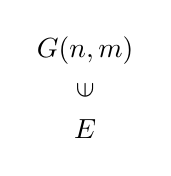
\begin{tikzpicture}[baseline=(g.base)]
\node (g) at (0,0) {$G(n,m)$};
\node[rotate=90] at (0,-0.5) {$\in$};
\node at (0,-1) {$E$};
\end{tikzpicture}
\end{adjustbox}
\qquad $e_1,\ldots,e_n$ — базис в $R^n$
\begin{equation*}
\tau_E=(Pe_1,\ldots,Pe_n)
\end{equation*}
Какова топ. страта в $G(n,m)$, где $\tau_E$ имеет заданный
комбинат. тип?

\noindent $2^{\circ}.$ Комбинат. теория выпуклых многогранников в $R^n$.

2 многогранника $V_1,V_2$ с упорядоч. (занумер.) вершинами
($n$ штук) [зачёркнуто: \Incomplete{GELFAND-P001229}{cancelled-type}{Зачёркнутый фрагмент после «(n штук)» не поддаётся надёжному чтению.}] имеют одинак. комбинат. тип, если
грани соответствуют друг другу.

Грассманизация задачи.

В $R^n$ рассм. подпр-во ($m$-мерное) $E$
\begin{equation*}
S=\omega(e_1,\ldots,e_n)\text{ — симплекс}
\end{equation*}
Проекция $S$ на $E$ — многогранник (выпуклый)

\underline{Упр.:} получ. комбинаторно любой многогранник разм. $m$ с $n$ вершинами

На $G(n,m)$ рассм. разбиение на подмн-ва, где несомые \Unclear{GELFAND-P001229}{subspace-abbreviation}{подпр-вм / подпр-вом}
многогранники комбинаторно эквивалентны.

Какова топология этих кусков?

\noindent $3^{\circ}.$
\begin{equation*}
\begin{pmatrix}
x_{11}&\cdots&x_{1n}\\
x_{21}&\cdots&x_{2n}\\
x_{31}&\cdots&x_{3n}
\end{pmatrix}
\qquad
\begin{pmatrix}
x'_{11}&\cdots&x'_{1n}\\
x'_{21}&\cdots&x'_{2n}\\
x'_{31}&\cdots&x'_{3n}
\end{pmatrix}
\text{ — 2 матрицы }3\times n
\end{equation*}
\SourceFigure{GELFAND-P001229}{matrix-hatching}{Под третьей строкой первой матрицы проведена горизонтальная черта и ниже — косая петлеобразная штриховка внутри продлённых скобок; вторую матрицу такая штриховка не сопровождает.}

Пусть все миноры $\ne0$ и имеют одинаковые знаки для $x$ и $x'$.

Сущ. ли гомотопия $x(t)$ матриц с $x(0)=x$, $x(1)=x'$

\SourcePage{GELFAND-P001230}{15}
в этом же классе?
\begin{gather*}
n\le7\ \Rightarrow\ \text{можно}\\
n=19\ \Rightarrow\ \text{нельзя!}\qquad\text{(Н.Е. Мнёв)}
\end{gather*}
Конфигурации имеют смысл и в $RP^n$ и нужно \Unclear{GELFAND-P001230}{configuration-end}{дополнить / дополнять}.

Надо \Unclear{GELFAND-P001230}{consequences-verb}{получать / пощупать} следствия (\Unclear{GELFAND-P001230}{consequences-parenthesis}{проектированности / проектируемости / ориентированности}) и есть аксиома,
сколько их надо брать, чтобы было достаточно.

Топология может быть как у любого алгебр. мн-зия!

(Это над $R$)

Над $C$ аналогом является вычисление $\pi_1$.

Интересно, что является выпуклым аналогом над $C$.

\underline{Теор. Стейница}: характеризация 1-мерн. остова вып. многогранника

(см. любой учебник вып. геом.) (в $R^3$)

\underline{Следствие}: пр-во многогр. данного комбинат. типа в $R^3$ стягиваемо.

\underline{Но}: В $R^4$ уже сущ. даже уже симплициальные многогранники
с более или менее любой [зачёркнуто: \Incomplete{GELFAND-P001230}{topology-cancel}{Зачёркнутое слово между «любой» и «топологией» не прочитано.}] топологией комбинат. типа.

\underline{Задача}: хотим на мн-зии построить поле многогранников! (в каждом
кас. пр-ве). была [зачёркнуто: \Incomplete{GELFAND-P001230}{classification-cancel}{Зачёркнутый фрагмент между «была» и «классифик.» не прочитан.}] классифик. задача для этой.

\underline{Матроиды} \Unclear{GELFAND-P001230}{matroid-mark}{м. / М.}. Дана решётка. Она наз. \underline{геометрич.} \underline{решёткой},
если она\quad 1) Полумодулярна

\hspace{3em}2) Конечная ($\forall$ элемент $=\sup$ конечн. числа атомов)

[Под этой строкой:] атомы — след. за нулём

Конфигур. — геом. решётка.

Обратно, пусть дана геом. решётка. Когда она зад. конфигур.?

\SourceFigure{GELFAND-P001230}{fano-diagram}{(1) Треугольник с тремя внутренними прямыми, идущими от вершин к отмеченным точкам противоположных сторон; они пересекаются в отмеченной центральной точке. Всего видны семь точек. Стрелок, буквенных меток и отдельной окружности не видно.}

(конфигур. Фано)\qquad над $R,Z$ не реализуется.

Верное предст. решётки $=$ её отображение
\begin{equation*}
a:\Gamma\longrightarrow\mathcal L(F^n)\text{ — реш. подпр-в,}
\end{equation*}
такое что
\begin{equation*}
\gamma_1<\gamma_2\ \Rightarrow\ a(\gamma_1)<a(\gamma_2)
\end{equation*}
и $\sup$ сохраняется

(1) не реализуется [зачёркнуто: \Unclear{GELFAND-P001230}{realization-cancel}{нечитаемый зачёркнутый знак}] над $R$, но над $Z_2$ реализу.

\SourcePage{GELFAND-P001231}{unlabelled}
Верное предст. есть у конфигур. (1):
\begin{equation*}
?\qquad m=4,\quad E,\quad \underline F,\quad \underline{R^6}
\end{equation*}
Зад. о реализуемости $\Leftrightarrow$ зад. о реш. системы алгебраических ур-в.

\underline{Перв. раб. по структурам} (по Гельфанду)

Дедекинд: придумал

Курош, Оре.

фон Нейман;

Гельфанд, Пономарёв;

[На левом поле: \underline{Доб. Вершика:}]
\underline{Пудлак и Тум} (Чехи): всякая конечная решётка вкладывается
в решётку разбиений конечного мн-ва (очень трудная теорема).

($\inf$ и $\sup$ — [зачёркнуто: \Incomplete{GELFAND-P001231}{inf-sup-cancel}{Зачёркнутое слово после «inf и sup —» не прочитано.}] пересеч. и объед.)

0 — разб. на точки.

\bigskip
\underline{Фейгин Б.}\qquad \underline{О струнах} [зачёркнуто: \Unclear{GELFAND-P001231}{string-heading-cancel}{зачёркнутый вертикальный знак; чтение не установлено}] (продолжение).

\underline{Операторная теория струн.}

\underline{Дуальные амплитуды.} Рассм. столкновение частиц

\begin{center}
\begin{adjustbox}{max width=\linewidth}
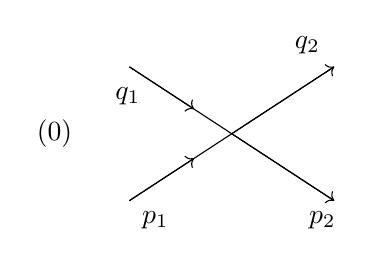
\begin{tikzpicture}
\node at (-2.25,0) {(0)};
\draw (-1.3,-0.85)--(1.3,0.85);
\draw (-1.3,0.85)--(1.3,-0.85);
\draw[->] (-1.3,-0.85)--(-0.48,-0.314);
\draw[->] (-1.3,0.85)--(-0.48,0.314);
\draw[->] (0,0)--(1.3,0.85);
\draw[->] (0,0)--(1.3,-0.85);
\node at (-0.97,-1.1) {$p_1$};
\node at (-1.32,0.48) {$q_1$};
\node at (0.96,1.12) {$q_2$};
\node at (1.15,-1.1) {$p_2$};
\end{tikzpicture}
\end{adjustbox}
\end{center}
Массы пусть все одинаковы и полный импульс $=0$

Всё — векторы в пр-ве/времени
\begin{equation*}
\begin{cases}
p_1+q_1=p_2+q_2,\\
p_1^2=q_1^2=p_2^2=q_2^2=m^2
\end{cases}
\qquad p_j,q_j\in R^4.
\tag{1}
\end{equation*}
Пусть дана $S$-матрица, характериз. это столкновение,
\begin{equation*}
S(p_1,q_1,p_2,q_2)
\tag{2}
\end{equation*}
Переменные Мандельстама:
\begin{equation*}
\begin{cases}
s=(p_1+q_1)^2,\\
t=(p_1-p_2)^2\\
u\ \text{[зачёркнуто: \ReaderApparatusRef{1}{1}]}=(p_1-q_2)^2
\end{cases}
\tag{3}
\end{equation*}
[Справа от (3):] (Заданы релятивистски инвариантные попарные скал. произведения)

зависим.:
\begin{equation*}
s+t+u=4m^2
\tag{4}
\end{equation*}
Зададим $A(s,t)$ ($=$ выражение $S$ через $s,t$)

Требование:
\begin{equation*}
1)\quad A\text{ аналитична по }s,t\ \text{[зачёркнуто: \ReaderApparatusRef{2}{1}]}
\tag{5}
\end{equation*}


\ReaderNotesStart{GELFAND-P001231}
\ReaderNote{1}{\Unclear{GELFAND-P001231}{mandelstam-u-cancel}{зачёркнутый знак}}
\ReaderNote{2}{\Unclear{GELFAND-P001231}{analytic-tail}{зачёркнутый знак после t}}
\ReaderNotesEnd
\SourcePage{GELFAND-P001232}{16}
2) $A$ симметрична по $s,t$ (независ. от порядка)

3) При фиксир. $t$ ф-я $A(s,t)$ имеет по $s$ только простые
полюса, причём [вписано между словами: 4)] места полюсов не зависят от $t$. Обычно пишут:
\begin{equation*}
A(s,t)=\sum_{n=0}^{\infty}\frac{R_n(t)}{n-\alpha(s)}
\tag{6}
\end{equation*}
5) $R_n(t)$ — многочлен

График $\alpha(s)$ наз. траекторией Редже.

Оказ., что из 1)—5) однозначно находим вид ф-и $A$:
\begin{equation*}
A(s,t)=\frac{\Gamma(-\alpha(s))\Gamma(-\alpha(t))}{\Gamma(-\alpha(s)-\alpha(t))}
=B(-\alpha(s),-\alpha(t))
\tag{7}
\end{equation*}
Из анализа экспер. данных вытекает, что
\begin{equation*}
\alpha(s)\text{ — линейная ф-я}
\tag{8}
\end{equation*}
$A$ наз. амплитудой Венециано, или дуальной амплитудой, а
усл. 1)—5) наз. \underline{условиями дуальности}.

Операторный метод: хотим записать $A(s,t)$ как опер. среднее
\begin{equation*}
\langle0|V(t)V(s)|0\rangle,
\tag{9}
\end{equation*}
где $\langle0|$ — вак. вектор в каком-то пр-ве, $V(t)$ — операторы.

Другая запись (7):
\begin{equation*}
S(p_1,p_2,p_3,p_4)=\int_0^1
x^{-2\langle p_1,p_2\rangle}(1-x)^{-2\langle p_2,p_3\rangle}
(x(1-x))^{-1-m^2}\,dx
\tag{10}
\end{equation*}
Здесь

\SourceFigure{GELFAND-P001232}{amplitude-arrow-convention}{(11) Четыре раздельных стрелки: слева сверху $p_2$ направлена вниз-вправо, слева снизу $p_1$ — вверх-вправо; справа сверху $p_3$ направлена вверх-вправо, справа снизу $p_4$ — вниз-вправо. Общая вершина не нарисована; около нижней правой стрелки есть дополнительное чернильное пятно.}
\begin{equation*}
p_1+p_2+p_3+p_4=0.
\end{equation*}
Аналогично можно писать амплитуды для большего числа частиц,
например:
\begin{equation*}
A(p_1,p_2,p_3,p_4,p_5)\cong\int\int_0^1
x^{\cdots}y^{\cdots}(1-x)^{\cdots}(1-y)^{\cdots}(1-xy)^{\cdots}\,dx\,dy
\tag{12}
\end{equation*}
Эта амплитуда уже не вычислена в общем виде, только при
нек-рых спец. значениях \underline{скал. произведений}.

Пр-во порождено \Unclear{GELFAND-P001232}{finite-oscillators}{конечным} набором осцилляторов, к-рые соед.
как в струне. Конечным числом обойтись нельзя!

Рассм. алгебру с образующими
\begin{equation*}
a_m^\mu,x^\mu,\quad \mu=0,1,\ldots,d,\quad
\text{[зачёркнуто: \ReaderApparatusRef{1}{2}]}
\tag{13}
\end{equation*}
где $d$ — разм. пр-ва


\ReaderNotesStart{GELFAND-P001232}
\ReaderNote{1}{\Incomplete{GELFAND-P001232}{generators-cancel}{Зачёркнутое выражение после d в (13) не прочитано.}}
\ReaderNotesEnd
\SourcePage{GELFAND-P001233}{unlabelled}
\begin{equation*}
[a_m^\mu,a_n^\nu]=m g^{\mu\nu}\delta_{m,-n}
\tag{14}
\end{equation*}
$m,n$ — целые числа
\begin{equation*}
a_0^\mu=p^\mu
\tag{15}
\end{equation*}
\begin{equation*}
[x^\mu,p^\nu]=i g^{\mu\nu}
\tag{16}
\end{equation*}
\begin{equation*}
[x^\mu,a_m^\nu]=0,\quad m\ne0
\tag{17}
\end{equation*}
Смысл образующих $x^\mu,a_m^\mu$:

[Зачёркнуто: $p^\mu$ — \Incomplete{GELFAND-P001233}{coordinates-cancel}{Продолжение зачёркнутого фрагмента после p с верхним μ не прочитано.}]
$(x^\mu,p^\mu)$ — коорд. и импульс центра тяжести летящей
струны, $a_m^\mu$ — разлож. в ряд Фурье всего остального.

Положим:
\begin{equation*}
P^\mu(\theta)=\sum_{-\infty}^{+\infty}a_m^\mu e^{-im\theta},
\tag{18}
\end{equation*}
(импульс точки с парам. $\theta$)
\begin{equation*}
Q^\mu(\theta)=x^\mu+a_0^\mu\theta+
 i\sum_{\substack{n=-\infty\\n\ne0}}^{\infty}\frac1n
\text{\ReaderApparatusRef{1}{1}}\,e^{-in\theta}
\tag{19}
\end{equation*}
Тогда выполнены коммутационные соотношения:
\begin{equation*}
[Q_\mu(\theta),P_\nu(\theta')]=2\pi i g_{\mu\nu}\delta(\theta-\theta')
\tag{20}
\end{equation*}
\begin{equation*}
[P_\mu(\theta),P_\nu(\theta')]=2\pi i g_{\mu\nu}\delta'(\theta-\theta')
\tag{21}
\end{equation*}
\begin{equation*}
[Q_\mu(\theta),Q_\nu(\theta')]=-\pi i g_{\mu\nu}\varepsilon(\theta-\theta'),
\tag{22}
\end{equation*}
где $\varepsilon$ — ф-я \Unclear{GELFAND-P001233}{heaviside-convention}{Хевисайда}
\begin{equation*}
L_m\overset{\mathrm{def}}{=}\frac1{4\pi}\int_0^{2\pi}
e^{im\theta}:P^2(\theta):\,d\theta
\tag{23}
\end{equation*}
Тогда получ. представление алгебры Вирасоро
\begin{equation*}
[L_m,L_n]=(m-n)L_{m+n}+\frac d{12}(m^3-m)\delta_{m,-n}
\tag{24}
\end{equation*}
\Unclear{GELFAND-P001233}{central-dimension}{$\frac{d}{12}(m^3-m)\delta_{m,-n}$}

\underline{Упражнение}: проверить это.

Кстати,
\begin{equation*}
L_0=\frac12a_0^2+\sum_{n=1}^{\infty}a_{-n}a_n
\tag{25}
\end{equation*}


\ReaderNotesStart{GELFAND-P001233}
\ReaderNote{1}{\Unclear{GELFAND-P001233}{fourier-index}{$a_n^\mu$ / $a_m^\mu$}}
\ReaderNotesEnd
\SourcePage{GELFAND-P001234}{17}
\begin{equation*}
2L_m=:\sum_{r+s=m}a_r a_s:
\tag{26}
\end{equation*}
\underline{Вертексный оператор}: положим
\begin{equation*}
V(k,\theta)=\exp\langle ik,Q(\theta)\rangle,
\tag{27}
\end{equation*}
где $k$ — вектор, тогда
\begin{equation*}
V(k)=V(k,0)=
\exp\left\langle k,\sum_{n=1}^{\infty}\frac{a_{-n}}n\right\rangle
\underbrace{\exp(ikx)}_{\text{[вставлено над строкой]}}
\exp\left\langle-k,\sum_{n=1}^{\infty}\frac{a_n}n\right\rangle
\tag{28}
\end{equation*}
и
\begin{equation*}
V(k,\theta)=\exp(i\theta L_0)V(k)\exp(-i\theta L_0).
\tag{29}
\end{equation*}
Далее,

[Зачёркнуто перед (30): \Incomplete{GELFAND-P001234}{commutator-cancel}{Зачёркнутое выражение перед коммутатором (30) не прочитано.}]
\begin{equation*}
[L_n-L_0,V(k)]=\frac{nk^2}2V(k).
\tag{30}
\end{equation*}
Рассмотрим серию взаимодействий:
\begin{center}
\begin{adjustbox}{max width=\linewidth}
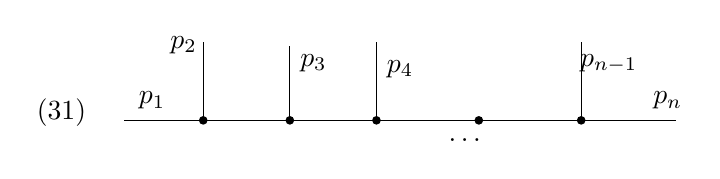
\begin{tikzpicture}
\node at (-0.8,0.1) {(31)};
\draw (0,0)--(7,0);
\draw (1,0)--(1,1);
\draw (2.1,0)--(2.1,0.95);
\draw (3.2,0)--(3.2,1);
\draw (5.8,0)--(5.8,1);
\fill (1,0) circle (0.055);
\fill (2.1,0) circle (0.055);
\fill (3.2,0) circle (0.055);
\fill (4.5,0) circle (0.055);
\fill (5.8,0) circle (0.055);
\node at (0.35,0.25) {$p_1$};
\node at (0.75,0.95) {$p_2$};
\node at (2.4,0.73) {$p_3$};
\node at (3.5,0.65) {$p_4$};
\node at (6.15,0.72) {$p_{n-1}$};
\node at (6.9,0.25) {$p_n$};
\node at (4.32,-0.25) {$\ldots$};
\end{tikzpicture}
\end{adjustbox}
\end{center}
и по такой картинке построим амплитуду:
\begin{equation*}
\langle0|V(p_2)D(s_2)V(p_3)D(s_3)\ldots D(s_{n-2})V(p_{n-1})|0\rangle,
\tag{32}
\end{equation*}
где $p$ — то же самое, что и $k$,
\begin{equation*}
\begin{aligned}
s_2&=(p_2+p_1)^2\\
s_3&=(p_3+p_2+p_1)^2,\\
&\ldots
\end{aligned}
\tag{33}
\end{equation*}
\begin{equation*}
D(s)=\int_0^1 x^{L_0-\alpha(s)-1}(1-x)^{\alpha(0)-1}\,dx,
\tag{34}
\end{equation*}
где $\alpha(s)$ — линейная ф-я (траектория Редже).

(32) — дуальная амплитуда; она должна совпадать с $A$,
когда 4 вершины.

Разложим $V(k,\theta)$ в ряд Фурье:
\begin{equation*}
V(k,\theta)=\sum V_n(k)e^{-in\theta}.
\tag{35}
\end{equation*}
Имеются операторы $a_i^\mu$ и $a_0^\mu$ и вакуумные векторы
$|0,p\rangle$, удовлетв. условию

\SourcePage{GELFAND-P001235}{unlabelled}
\begin{equation*}
a_i^\mu|0,p\rangle=0,\quad\text{если }i>0,
\tag*{$(36)_i$}
\end{equation*}
\begin{equation*}
a_0^\mu|0,p\rangle=
\text{[зачёркнуто: \ReaderApparatusRef{1}{1}]}\ p^\mu\,
\text{[зачёркнуто: \ReaderApparatusRef{2}{1}]}\ |0,p\rangle.
\tag*{$(36)_0$}
\end{equation*}
(вакуумы занумерованы векторами импульса)

Получим пр-во
\begin{equation*}
\bigoplus_p H(p)
\tag{37}
\end{equation*}
Вертексный оператор действует так:
\begin{equation*}
V_n(k):H(p)\longrightarrow H(p+k).
\tag{38}
\end{equation*}
Коммутационные соотношения:

[Зачёркнуто: \Incomplete{GELFAND-P001235}{commutator-cancel}{Зачёркнутая запись под заголовком «Коммутационные соотношения» не прочитана.}]
\begin{equation*}
[a_m^\mu,V_n(k)]=V_{n+m}(k)\cdot k_\mu
\tag{39}
\end{equation*}
[Зачёркнуто: \Unclear{GELFAND-P001235}{vertex-cancel}{$V_n(k_1)|0,p\rangle$ / $V_1(k_1)|0,p\rangle$}] Положим
\begin{equation*}
\langle0,p+k_1+k|V_{-n}(k_2)V_n(k_1)|0,p\rangle=A_n\qquad\text{(это числа)}
\tag{40}
\end{equation*}
\Unclear{GELFAND-P001235}{bra-last-momentum}{$k$ без нижнего индекса}

Тогда
\begin{equation*}
\sum A_n z^n=(1-z)^{\langle k_1,k_2\rangle}.
\tag{41}
\end{equation*}
Это доказывается простым вычислением. Предлагается
проверить (41) в качестве упражнения.


\ReaderNotesStart{GELFAND-P001235}
\ReaderNote{1}{\Unclear{GELFAND-P001235}{vacuum-cancel-left}{нечитаемый зачёркнутый множитель}}
\ReaderNote{2}{\Unclear{GELFAND-P001235}{vacuum-cancel-right}{зачёркнутый знак}}
\ReaderNotesEnd
\SourcePage{GELFAND-P001236}{26}
\underline{18/XI–85г.}\qquad \underline{Сем. Гельфанда}

\underline{Б. Фейгин} (продолжение).

$L_i$ — образующие алг. Вирасоро; пусть есть большое пр-во, в к-ром действ.
эта алгебра

Соб. векторы $L_0=$ весовые векторы

$L_i$ действует в пр-ве весовых векторов из коммут. соотношений

(см. (24) на стр. 17 лев.)

Старший [зачёркнуто: \Unclear{GELFAND-P001236}{highest-cancel}{вектор?}] вес: вектор, к-рый нельзя уже повысить
\begin{equation*}
\widetilde{\mathcal H}=\{v\mid L_0v=v,\quad L_iv=0\ \text{при }i>0\}.\qquad\text{(вес 1)}
\tag{1}
\end{equation*}
\begin{equation*}
\overline{\mathcal H}=\{v\in\widetilde{\mathcal H},\quad v=L_i v',\ i<0\},
\tag{2}
\end{equation*}
[Справа:] здесь $v'$ — произв. весовой вектор из большого пр-ва.

(пр-во «спурионов» — назв. физиков, $\sim15$ лет назад)
\begin{equation*}
\mathcal H\overset{\mathrm{def}}{=}\widetilde{\mathcal H}/\overline{\mathcal H}
\tag{3}
\end{equation*}
\begin{equation*}
\prod_{i=1}^N a_{m_i}^{\mu_i}|0,p\rangle
\tag{4}
\end{equation*}
[Справа:] (пр-во состояний)

большой модуль над алг. Вирасоро
\begin{equation*}
L_{-1}v'=v\quad\Rightarrow\quad v'\text{ имеет вес 2}:\quad L_0v'=2v'
\tag{5}
\end{equation*}
\Unclear{GELFAND-P001236}{weight-two}{$L_{-1}v'=v;\quad L_0v'=2v'$}

Цель: факторизация отн. группы диффеом. во всём пр-ве, но
действует центр. расширение, и центр действ. нетривиально.

Предлаг. другая процедура получ. «инвар.» векторов: относит. половины
они инвар., затем факторизуем по действию других и отбрасываем.

Алг. Вирасоро исчезает, от неё остаётся пр-во инвариантов.

Хотим:

I. Построить пр-во, порожд. $d-2$ осцилляторами.

II. Док., что все векторы в $\widetilde{\mathcal H}/\overline{\mathcal H}$ имеют норму $>0$

(в исх. $d$-мерном это не так)

(отсутствие \underline{\Unclear{GELFAND-P001236}{tachyon-word}{тахионов}})

В размерности 26 это всё достигается.

\SourcePage{GELFAND-P001237}{unlabelled}
Вертексные операторы:
\begin{equation*}
X(p,z)=\exp\left(p_\mu\sum_{n=1}^{\infty}a_{-n}^\mu z^n\right)D_p
\exp\left(-p_\mu\sum_{n=1}^{\infty}\frac{a_n^\mu}{n}z^{-n}\right),
\tag{6}
\end{equation*}
\Unclear{GELFAND-P001237}{left-exponential-normalization}{$a_{-n}^{\mu}z^n$ без деления на $n$}

где операторы $D_p$ опред. ф-лами
\begin{equation*}
D_p|0,k\rangle=|0,k+p\rangle,\quad [D_p,a_n^\mu]=0,\ n\ne0.
\tag{7}
\end{equation*}
Корреляционная функция:
\begin{equation*}
\langle0,k+\sum p_i|X(z_1,p_1)\ldots X(z_n,p_n)|0,k\rangle
=\prod_{\text{\ReaderApparatusRef{1}{1}}}\left(1-\frac{z_j}{z_i}\right)^{\langle p_i,p_j\rangle}
\tag{8}
\end{equation*}
Разлагая $X(z,p)$ в ряд, получим:
\begin{equation*}
X(z,p)=\sum X_i(p)z^i
\tag{9}
\end{equation*}
(это определение операторов $X_i(p)$)

Хотим построить 24 осциллятора.

Далее будут строиться операторы
\begin{equation*}
\int X(p,z)\frac{dz}{z},
\tag{10}
\end{equation*}
коммутирующие с алг. Вирасоро при $\langle p,p\rangle=2$.
\begin{equation*}
\begin{aligned}
&\text{На }R^{26}\text{ хотим иметь }p_1,\ldots,p_n:\quad\langle p_i,p_i\rangle=2\\
&\langle p_i,p_j\rangle=A_{ij}\in Z,\quad A_{ij}<0.
\end{aligned}
\tag{11}
\end{equation*}
[На левом поле: \Unclear{GELFAND-P001237}{cartan-margin-cancel}{зачёркнутый вертикальный знак}]

\Unclear{GELFAND-P001237}{cartan-diagonal}{$A_{ij}<0$}

Тогда операторы
\begin{equation*}
e_i=\int X(p_i,z)\frac{dz}{z},\quad f_i=\int X(-p_i,z)\frac{dz}{z}
\tag{12}
\end{equation*}
порождают на пр-ве действие алгебры Каца–Муди с матрицей
Картана $A_{ij}$; при этом надо ещё положить
\begin{equation*}
h_i|0,k\rangle=\langle k,p_i\rangle|0,k\rangle
\tag{13}
\end{equation*}
\underline{Читать}: ст. \underline{МакДональда} (начало), \underline{Sem. Bourbaki};

учить алгебры Ли по ней.

[На левом поле: И.М.Г.]
В самой большой простой конечной группе $\sim10^{54}$ элементов; она
связана со струнами!

[Приписано справа:] (монстр «Лунное сияние»)

Moonshine

(есть раб. Френкель, Леповский и кто-то ещё)

Как-то получ. фунд. предст. алг. Каца–Муди.


\ReaderNotesStart{GELFAND-P001237}
\ReaderNote{1}{\Unclear{GELFAND-P001237}{product-index}{$j>1$ / $j>i$}}
\ReaderNotesEnd
\SourcePage{GELFAND-P001238}{27}
В $R^{26}$ рассмотрим метрику $\langle-1,1,1,\ldots,1\rangle$,

[Зачёркнуто: \Unclear{GELFAND-P001238}{null-cancel-before}{нулев?}] вектор длины 0, [зачёркнуто: \Incomplete{GELFAND-P001238}{null-cancel-after}{Зачёркнутое слово после «вектор длины 0» не прочитано.}]

[Перед следующей строкой: \Unclear{GELFAND-P001238}{null-marks}{два вертикальных знака; чтение не установлено}] 24 осциллятора

(Обзор \Unclear{GELFAND-P001238}{schwarz-initial}{Д. / D. / Дж.} Шварца 1973 года).

\begin{center}—\quad .\quad —\end{center}

$R^d$ с индефин. метрикой и пусть дан вектор $p$ с $\langle p,p\rangle=0$

[Под «метрикой»:] (Минковского; 1 минус)

Положим
\begin{equation*}
U_n(v)=\int v(z)X(np,z)\frac{dz}{z},
\tag{14}
\end{equation*}
где $v\in R^d$, $v=\sum v_i e_i$, $v(z)=\sum v_\mu a_n^\mu z^n$

Пусть
\begin{equation*}
v^1,v^2,\ldots,v^{d-2}\text{ — такие, что }\langle v^i,p\rangle=0
\tag{15}
\end{equation*}
[Над зачёркнутым знаком вставлено «и»:] и [зачёркнуто: \Unclear{GELFAND-P001238}{basis-cancel-left}{зачёркнутый знак под вставленным «и»}]
$v^1,v^2,\ldots,v^{d-2},p$ — базис в пр-ве
[зачёркнуто: \Incomplete{GELFAND-P001238}{basis-cancel-right}{Зачёркнутое слово между «в пр-ве» и фигурной скобкой не прочитано.}] $\{x:\langle x,p\rangle=0\}$.

Положим
\begin{equation*}
b_n^\mu=U_n(v^\mu);
\tag{16}
\end{equation*}
$b_n^\mu$ образуют алг. Гейзенберга $\Rightarrow$ осцилляторы.

Они порождают всё пр-во.

Есть ещё обзор Грина и Шварца (томик Physics Reports)

\bigskip
\underline{Зелевинский А.}\qquad \underline{Клетки}
[над строкой вставлено: \underline{(и многочлены)}]
\underline{Шуберта и когомологии мн-зий флагов.}

О работах \underline{A. [зачёркнуто: \Unclear{GELFAND-P001238}{lascoux-cancel}{зачёркнутый инициал}] Lascoux},
\underline{M.-P. Schützenberger}

(клетки Шуберта и когом. грассм. мн-зий; мн-зий флагов)

продолж. раб. Берншт., И.М.Г. и С.И.Г. УМН, 1973, 28:3, 3–26.

$X$ — мн-зие полных флагов в $V^n$ (флаги подпр-в)

[Под $X$, над (1): \Unclear{GELFAND-P001238}{flag-relation}{Н-образный знак}]
\begin{equation*}
\{V^1\subset V^2\subset\ldots\subset V^n\}
\tag{1}
\end{equation*}
Когомологии опис. 2-мя способами

$1^{\circ}.$ \underline{Borel}
\begin{equation*}
H^*(X,Q)=Q[x_1,\ldots,x_n]/J
\end{equation*}
Идеал $J$ порождён симметр. многочленами без своб. члена

$2^{\circ}.$ Базис в гомологиях $H_*(X,Q)$ сост. клетки Шуберта $(c_w)$

$w$ — перестановка чисел от 1 до $n$
\SourcePage{GELFAND-P001239}{unlabelled}
\begin{equation*}
\begin{array}{cccc}
1&2&\ldots&n\\
i_1&i_2&\ldots&i_n
\end{array}
\end{equation*}
Рассм. фикс. полный флаг
\begin{equation*}
F=(\langle e_1\rangle,\ \langle e_1,e_2\rangle,\ \langle e_1,e_2,e_3\rangle,\ldots,\ \langle e_1,e_2,\ldots,e_n\rangle).
\end{equation*}
Подействуем на него перест. $w$:
\begin{equation*}
F_w=(\langle e_{w(1)}\rangle,\ \langle e_{w(1)},e_{w(2)}\rangle,\ldots)
=(\langle e_{i_1}\rangle,\ \langle e_{i_1},e_{i_2}\rangle,\ldots).
\end{equation*}
[Зачёркнуто: \Unclear{GELFAND-P001239}{cancel-cell}{Клетка?}. Над зачёркнутым вставлено: $(C_w)\overset{\mathrm{def}}{=}$.]
[Подчёркнуто: (Траектория флага $F_w$ под действием лин. преобразований, сохраняющих флаг $F$).]
[Зачёркнуто: \Unclear{GELFAND-P001239}{cancel-after-orbit}{неразборчивое обозначение}.]
\begin{equation*}
\dim_{\mathbb C} c_w=\ell(w)\text{ — число инверсий в }w.
\end{equation*}
Двойств. базис в когомологиях:
\begin{equation*}
P_w\in H^{2\ell(w)}(X;\mathbb Q).
\end{equation*}
Б.-Г.-Г. нашли явные ф-лы для $P_w$ в реализ. Бореля — многочлены (!).
[Под первым словом «многочлены»: $(\operatorname{mod}J)$.]
[Зачёркнуто: \Unclear{GELFAND-P001239}{middle-cancel}{неразборчиво}.]
Теперь их подняли и получились просто многочлены: их степени
\begin{equation*}
\operatorname{deg} P_w=\ell(w).
\end{equation*}
\begin{equation*}
P_{\mathrm{id}}=1.
\end{equation*}
\begin{equation*}
w_0=(n,n-1,\ldots,1).
\end{equation*}
Тогда
\begin{equation*}
\operatorname{deg} P_{w_0}=\frac{n(n-1)}{2}.
\end{equation*}
Неоднозначно выб., выберем
\begin{equation*}
P_{w_0}=x_1^{n-1}x_2^{n-2}\ldots x_{n-1}.
\end{equation*}
(У Б.-Г.-Г.: $\displaystyle\prod_{i<j}(x_i-x_j)$ — то же самое $\operatorname{mod}$ идеала.)
\Unclear{GELFAND-P001239}{bgg-normalization}{В рукописи у произведения нет нормирующего множителя.}

Или: $\displaystyle\frac{\rho^{n(n-1)/2}}{\frac{n(n-1)}{2}!}$, где $\rho=(n-1)x_1+(n-2)x_2+\ldots$

Остальные выражаются:
\begin{equation*}
P_w=A_{w_0w^{-1}}P_{w_0},
\end{equation*}

\SourcePage{GELFAND-P001240}{28}
$A_w$ — опер., отвеч. перест.
\begin{equation*}
w=(i_1,i_1+1)(i_2,i_2+1)\ldots(i_{\ell(w)},i_{\ell(w)+1})
\end{equation*}
(произв. инверсий).
\Unclear{GELFAND-P001240}{top-last-index}{В последнем множителе $+1$ написано на уровне индекса: $i_{\ell(w)+1}$ или $i_{\ell(w)}+1$.}

\begin{equation*}
A_{(i,i+1)}=
\frac{p(x_1,\ldots,x_i,x_{i+1},\ldots,x_n)-p(x_1,\ldots,x_{i+1},x_i,\ldots,x_n)}{x_{i+1}-x_i}.
\end{equation*}
[После знака равенства, перед дробью, зачёркнуто:
\Unclear{GELFAND-P001240}{cancel-polynomial}{$p(x_1,\ldots$; далее неразборчиво}.]
\Unclear{GELFAND-P001240}{fraction-sign}{Знаменатель в рукописи: $x_{i+1}-x_i$.}

Оператор
\begin{equation*}
A_w=A_{(i_1,i_1+1)}\ldots A_{(i_{\ell(w)},i_{\ell(w)+1})}
\end{equation*}
\Unclear{GELFAND-P001240}{operator-last-index}{В последнем индексе оператора: $i_{\ell(w)+1}$ или $i_{\ell(w)}+1$.}
опрд. корректно (не зав. от разложения в произведение инверсий).
Он и использован в ф-ле.

\underline{Усл. симметрии}.

$P_w$ симметричен отн. $x_i,x_{i+1}$, если $(i,i+1)$ не явл. инверсией для $w$.

\SourcePage{GELFAND-P001241}{35}
\underline{25/XI-85 г.}\qquad \underline{Сем. Гельфанда.}

\underline{Фейгин} (продолжение). (О струнах).

Образующие алгебры Вирасоро:
\begin{equation*}
L_i=:\sum_{m+n=i}g_{\mu\nu}a_m^\mu a_n^\nu:\tag{1}
\end{equation*}
$:\quad:$ обеспечивают корректность опред. оператора и дают только добавление постоянной.

\underline{И.М.Г.:} Что нужно, чтобы была операция $:\quad:$? Здесь она приводит к появлению алг. Вирасоро. Что если взять решетку или тор? Что на сфере?
\begin{equation*}
[L_i,L_j]=(i-j)L_{i+j}+\delta_{i,-j}\frac{i^3-i}{12}\,c\tag{2}
\end{equation*}
\begin{equation*}
p^\mu(t)=\sum a_m^\mu e^{-imt},\qquad
q^\mu(t)=\sum_{m\ne0}\frac{a_m^\mu}{m}e^{-imt}+q_0^\mu\tag{3}
\end{equation*}
\begin{equation*}
[x^\mu,a_m^\nu]=0,\quad m\ne0,
\end{equation*}
\begin{equation*}
[x^\mu,a_0^\nu]=g^{\mu\nu},
\end{equation*}
\begin{equation*}
x^\mu(t)=x^\mu+\sum_{n\ne0}\frac1n\bigl(a_n^\mu e^{-int}\bigr).
\end{equation*}
\underline{И.М.Г.} В классич. теории:
\begin{equation*}
L_n=e^{int}\frac{d}{dt}.
\end{equation*}
Квант. механика соотв. одномерному расширению классич. теории: ср. $[\frac{d}{dx},x]=1$.

(4) $\mathcal H_p$ — модуль, порожденный высш. вектором $|p\rangle$.

[Справа: (\Unclear{GELFAND-P001241}{module-margin}{зачёркнутое обозначение неразборчиво} $a_m^\mu$ и тд). Над зачёркнутым вставлено «(примен.)», проведена линия к месту вставки.]

[Между строками:] Это модуль над алг. Вирасоро.

(5) Структура его зависит только от
\Unclear{GELFAND-P001241}{module-norm}{$\langle p,\xi p\rangle$? Между запятой и вторым $p$ есть дополнительный знак}; по определению
\begin{equation*}
a_m^\nu|p\rangle=0,\quad m>0,\qquad
 a_0^\nu|p\rangle=p^\nu|p\rangle\tag{6}
\end{equation*}
(5) $\mathcal H_p\cong\mathcal H_{p'}$, если $\langle p,p\rangle=\langle p',p'\rangle$.
$\Vert$ Обозначим его $\mathcal H_{\langle p,p\rangle}$.

Рассмотрим
\begin{equation*}
\bigoplus_{\langle p,p\rangle\in\mathbb R}\mathcal H_{\langle p,p\rangle}\tag{7}
\end{equation*}

\SourcePage{GELFAND-P001242}{unlabelled}
Определим из [зачёркнуто: \Unclear{GELFAND-P001242}{cancel-before-module}{неразборчивый знак}] модуля (7) пр-во физических состояний,
как делалось [зачёркнуто: \Unclear{GELFAND-P001242}{cancel-before-above}{неразборчивый знак}] выше (стр. (26)).
Конструкция зависит [над строкой вставлено: только] от
[зачёркнуто: \Unclear{GELFAND-P001242}{cancel-before-action}{определения?}] действия алг. Вирасоро.

(8) \underline{Теорема}. (о духах).

1) Сущ. система осцилляторов $b_m^\mu$, $m\ne0$, $\mu=1,2,\ldots,24$
со станд. коммут. соотн.
\Unclear{GELFAND-P001242}{oscillator-prefix}{д?}
на пр-ве [зачёркнуто: \Unclear{GELFAND-P001242}{cancel-physical-space}{неразборчивое обозначение}; над строкой вставлено: физ. состояний]
и такая, что
\begin{equation*}
[L_i,b_m^\mu]=0.
\end{equation*}
$b_m^\mu$ можно постр. из $a$.

2) $\exists$ в пр-ве физ. сост. [сверху вставлено: $\widetilde{\mathcal H}$] выс. вектор $|0\rangle$,
и $\widetilde{\mathcal H}$ порождается векторами $|0\rangle$ и опер. $b_n^\nu$.
Это только при \underline{$d=26$}.

3) В $\widetilde{\mathcal H}$ имеется естеств. квадр. форма, наследуемая с пр-ва (7),
и она на $\widetilde{\mathcal H}$ положит. определена.
\begin{equation*}
X(p,z)=\exp\left(p_\mu\sum_{n=1}^{\infty}\frac{a_{-n}^\mu}{n}z^n\right)
D_p\exp\left(-p_\mu\sum_{n=1}^{\infty}\frac{a_n^\mu}{n}z^{-n}\right),\tag{9}
\end{equation*}
Здесь $D_p$ опред. формулой
\begin{equation*}
D_p|k\rangle=|k+p\rangle,\tag{10}
\end{equation*}
[Зачёркнуто: а при этом.] Причём
\begin{equation*}
[D_p,a_n^\mu]=0,\quad n\ne0.\tag{11}
\end{equation*}
Коммутац. соотношения $X(p,z)$ и $a_n^\mu$: если
\begin{equation*}
X(p,z)=\sum X_j(p)z^j,
\end{equation*}
то
\begin{equation*}
[a_n^\mu,X_i(p)]=p^\mu X_{i+n}(p).\tag{12}
\end{equation*}
\Unclear{GELFAND-P001242}{mode-convention}{В разложении написано $z^j$, а в (12) — $X_{i+n}(p)$.}

\underline{Представление алгебры токов.}

Пр-во разм. $d$, рассм. в $\mathbb R^d$ решётку $Q$ (дискр. подгруппу),
счит., что $Q$ целочисленна и унимодулярна: есть такой базис
\begin{equation*}
e_1,\ldots,e_d,\quad\text{что }\langle e_i,e_j\rangle\text{ целочисл. и }\det\langle e_i,e_j\rangle=1.\tag{13}
\end{equation*}
Чётная решётка:
\begin{equation*}
\forall\gamma\in Q:\quad\langle\gamma,\gamma\rangle\text{ — чётное}.\tag{14}
\end{equation*}

[Узкая полоса соседнего листа у правой границы кадра:]
\Unclear{GELFAND-P001242}{right-edge}{Сверху вниз видны обрезанные «(», «(», «(», «(», короткий вертикальный штрих и «(»; содержимое скобок за границей кадра.}

\SourcePage{GELFAND-P001243}{36}
(15) \underline{Корень решётки}: такой вектор $\gamma\in Q$, что $\langle\gamma,\gamma\rangle=2$.

(16) [Зачёркнуто: \Unclear{GELFAND-P001243}{cancel-before-these}{$Q$?}.]
Такие бывают начиная с размерности
[зачёркнуто: \Unclear{GELFAND-P001243}{cancel-before-eight}{неразборчиво}]
$8$
[зачёркнуто: \Unclear{GELFAND-P001243}{cancel-after-eight}{неразборчивый знак}], точнее,
[зачёркнуто: \Unclear{GELFAND-P001243}{cancel-before-only}{неразборчивый знак}]
только в размерности, делящейся на $8$.

\underline{Упражнение}: построить \underline{такую} решётку в $\mathbb R^8$.

$Q$ — решётка (пока не обязательно чётная).

\underline{Кстати:}
[Зачёркнуто: \Unclear{GELFAND-P001243}{aside-cancel}{и?}.]
Решётки корней групп серии $A,D,E$ облад. этим св-вом (14).

Рассм. функцию:
\begin{equation*}
\varepsilon:Q\times Q\longrightarrow\{\pm1\}\tag{17}
\end{equation*}
\begin{equation*}
\varepsilon(\alpha,\beta)\cdot\varepsilon(\beta,\alpha)=(-1)^{\langle\alpha,\beta\rangle},
\qquad\alpha,\beta\in Q;\tag{18}
\end{equation*}
\Unclear{GELFAND-P001243}{epsilon-parity}{Условие (18) и слова «пока не обязательно чётная» сохранены как в источнике.}
\begin{equation*}
\varepsilon(\alpha,\alpha)=-1\quad\text{если }\langle\alpha,\alpha\rangle=2.\tag{19}
\end{equation*}
$\Delta$ — мн-во корней решётки $Q$, т.е.
$\Delta=\{\gamma\in Q\mid\langle\gamma,\gamma\rangle=2\}$.

Пусть квадр. форма $\langle\ ,\ \rangle$ полож. определена.
Введём алгебру Ли:
\begin{equation*}
\mathfrak g=f+\sum_{\alpha\in\Delta}\mathbb Cx_\alpha,\tag{20}
\end{equation*}
где $f=\mathbb R^d\otimes\mathbb C=\mathbb C^d$.
\Unclear{GELFAND-P001243}{cartan-symbol}{Одинаковая петлеобразная буква в (20) и после «где» передана как $f$; возможно, это особое написание $\mathfrak h$.}

Зададим структуру алг. Ли на $\mathfrak g$ по формулам:
\begin{equation*}
[h,x_\alpha]=\langle h,\alpha\rangle x_\alpha;\tag*{$(21)_1$}
\end{equation*}
\begin{equation*}
[x_\alpha,x_\beta]=0\quad\text{если }\alpha+\beta\notin\Delta\cup\{0\};\tag*{$(21)_2$}
\end{equation*}
\begin{equation*}
[x_\alpha,x_\beta]=\varepsilon(\alpha,\beta)x_{\alpha+\beta}
\quad\text{если }\alpha+\beta\in\Delta;\tag*{$(21)_3$}
\end{equation*}
\begin{equation*}
[x_\alpha,x_{-\alpha}]=-\alpha.\tag*{$(21)_4$}
\end{equation*}
Это \Unclear{GELFAND-P001243}{construction-adjective}{весовая?} конструкция конечномерных простых алгебр.

Пусть теперь в конструкции, опис. выше, $p\in Q$,
$|p\rangle$ — вак. вектор, $\gamma\in\Delta$.
Рассмотрим вертексный оператор
\begin{equation*}
X^\varepsilon(\gamma,z)=X(\gamma,z)\cdot\varepsilon_\gamma;\tag*{$(22)_1$}
\end{equation*}
где
\begin{equation*}
\varepsilon_\gamma|p\rangle=\varepsilon(\gamma,p)|p\rangle,\tag*{$(22)_2$}
\end{equation*}

\SourcePage{GELFAND-P001244}{unlabelled}
\begin{equation*}
[\varepsilon_\gamma,a_m^\mu]=0,\quad m\ne0.\tag*{$(22)_3$}
\end{equation*}
Теперь введём
\begin{equation*}
X^\varepsilon(\gamma,z)=\sum X_i^\varepsilon(\gamma)z^i.\tag{23}
\end{equation*}
В $\mathbb R^{24}$ есть спец. решетка (особая), к-рая встреч. здесь и в теории конечных простых групп.
Всего спорадических простых групп $26$.

(24) $\{X_n^\varepsilon(\gamma),a_n^\mu\}$ порождают
[над строкой вставлено: проективное] предст. алг. токов на окружности.
\begin{equation*}
[X_n^\varepsilon(\gamma_1),X_m^\varepsilon(\gamma_2)]=0,
\quad\text{если }\langle\gamma_1,\gamma_2\rangle>0\tag*{$(25)_1$}
\end{equation*}
\begin{equation*}
[X_n^\varepsilon(\gamma_1),X_m^\varepsilon(\gamma_2)]
=\varepsilon(\gamma_1,\gamma_2)X_{n+m}^\varepsilon(\gamma_1+\gamma_2),
\quad\text{если }\langle\gamma_1,\gamma_2\rangle=-1\tag*{$(25)_2$}
\end{equation*}
и другие [зачёркнуто: \Unclear{GELFAND-P001244}{cancel-other-relations}{неразборчивое слово}] соотн. пишутся.

В $\mathbb R^{26}$ выберем вектор $c$, такой что $\langle c,c\rangle=0$, и рассмотрим интегралы
\begin{equation*}
\int a(z)X(nc,z)\frac{dz}{z}\tag{26}
\end{equation*}
[У $a(z)$ зачёркнут верхний индекс:
\Unclear{GELFAND-P001244}{cancel-integrand-index}{$\mu$?}.]
[После интеграла зачёркнуто:
\Unclear{GELFAND-P001244}{cancel-after-integral}{$=b_n^\mu$?}.]

Здесь
\begin{equation*}
a(z)=\sum a_m z^m,\tag{27}
\end{equation*}
[У $a_m$ зачёркнут верхний индекс:
\Unclear{GELFAND-P001244}{cancel-mode-index}{$\mu$?}.]
где
\begin{equation*}
a_m=\sum\alpha_\mu a_m^\mu,\tag*{$(27)'$}
\end{equation*}
(28) а вектор $(\alpha_1,\ldots,\alpha_{26})$ ортогонален к $c$.

Положим
\begin{equation*}
b_n^\mu=\int a^\mu(z)X(nc,z)\frac{dz}{z}\tag{29}
\end{equation*}
\begin{equation*}
\langle\alpha,c\rangle=0.\tag{30}
\end{equation*}
Выберем $\alpha^1,\alpha^2,\ldots,\alpha^{24}$, чтобы вместе с $c$ они сост. базис
в пр-ве векторов, ортог. к $c$; подставляя их в $(27)'$, получим набор $a^\mu$ и далее $b_n^\mu$.

\SourcePage{GELFAND-P001245}{56}
\underline{16/XII-85 г.}\qquad \underline{Сем. Гельфанда}

\underline{С. П. Новиков.}

\underline{Солитонная теория 2-мерного оператора Шредингера.}

\underline{$n=2$}
\begin{equation*}
L=-\partial\bar\partial+U=-\Delta+U\tag{1}
\end{equation*}
не бывает пар Лакса:
\begin{equation*}
\frac{\partial L}{\partial t}=[A,L]
\quad\Rightarrow\quad
\text{завис. от }t\text{ — однопар. группа движ. }\mathbb R^2\tag{2}
\end{equation*}
1976\quad 1) Манаков УМН

\hspace{2em}2) Дубр., Крич., Нов. ДАН.

Разница с 1-мерным случаем.
\begin{equation*}
U(x)\to0\quad\text{при }|x|\to\infty;
\quad\Rightarrow\quad\text{возникает амп. рас. }S(k_1,k_2),
\quad |k_1|=|k_2|.\tag{3}
\end{equation*}
$x$ \Unclear{GELFAND-P001245}{scattering-dimension}{горизонтальный штрих и неразборчивый надстрочный знак}
$(n\text{ перем.})$.

[Справа:]
\Unclear{GELFAND-P001245}{scattering-pairs}{$\{(k_1,k_2),|k_1|=|k_2|\}$?}
$(2n-1)$ перем.
\begin{equation*}
n=2n-1\Leftrightarrow n=1.
\end{equation*}
Переопред. задача.

\underline{$n=2$}\quad $\Rightarrow$ огранич. на фикс. $|k_1|=|k_2|$ — тоже 2 перем.

Потребуем:
\begin{equation*}
\begin{cases}
\left(\dfrac{\partial L}{\partial t}-[A,L]\right)\psi=0,\\
L\psi=0
\end{cases}
\qquad(\text{или }L\psi=\varepsilon_0\psi)\tag{4}
\end{equation*}
или
\begin{equation*}
\frac{\partial L}{\partial t}=\underline{[A,L]+BL},
\qquad A,B\text{ — дифф. операторы}.\tag{5}
\end{equation*}
[Под подчёркнутой правой частью, со знаком равенства, поставленным вертикально:]
\begin{equation*}
C_1L+LC_2
\end{equation*}
Обр. зад. реш. с той же эффективностью.

(5) наз. 2-мерным аналогом ур-я Лакса.
При $n=2$ оно уже непротиворечиво.

$z=x+iy$, $\bar z$ и ещё $t$.

Надо начать с периодических задач (или квазипериодических).

$\Gamma$ — рим. пов. рода $g<\infty$, $\infty_1,\infty_2$ — 2 точки на $\Gamma$,

$P_1+\cdots+P_g$ — \Unclear{GELFAND-P001245}{divisor-adjective}{вхд.?} дивизор;
$w_1,w_2$ — лок. коорд. около $\infty_1,\infty_2$,

($P_j$ — другие точки, $\ne\infty_k$ и друг другу), $k_j=w_j^{-1}$.

\SourcePage{GELFAND-P001246}{unlabelled}
(6) Ищем соб. ф-ю $\Psi(x,y,P)$ со св-вами

[Под $P$ написано $\Gamma$, со стрелкой $\uparrow$ к $P$.]

1) $\psi$ мероморфна по $P$ вне $\infty_1$ и $\infty_2$.
[Справа: $(x,y$ и, возможно, $t$ — параметры).]

2) $g$ полюсов $P_j$, не зависящих от $(x,y)$

3)
\begin{equation*}
\psi\sim c_1(x,y)e^{ik_1z}(1+O(w_1)),\qquad\text{в окр. }\infty_1
\end{equation*}
\begin{equation*}
\psi\sim c_2(x,y)e^{ik_2\bar z}(1+O(w_2))\qquad\text{в окр. }\infty_2
\end{equation*}
(7) \underline{Калибр. преобр.}
\begin{equation*}
\begin{aligned}
c_1&\to cc_1\\
c_2&\to cc_2
\end{aligned}
\quad\bigg|\quad c=c(x,y)
\end{equation*}
не меняют ничего.

Будем считать $c_1\equiv1$ $\Rightarrow$ она станет единственной.

(8) \underline{Теорема} (ДКН, 1976) $\exists L$:
\begin{equation*}
L\psi=0,\qquad L=\partial\bar\partial+A(z,\bar z)\partial+B(z,\bar z),\tag{9}
\end{equation*}
где
\begin{equation*}
A=\bar\partial\ln c_2.\tag{10}
\end{equation*}
\Unclear{GELFAND-P001246}{derivative-convention}{В (9) после $A$ стоит $\partial$ без черты, в (10) — $+\bar\partial\ln c_2$; запись сохранена без согласования с асимптотиками (6).}

(11) $A,B$ — квазипериодич. для рим. пов. общ. положения.

(12) Магн. поле обяз. с [зачёркнуто: \Unclear{GELFAND-P001246}{magnetic-cancel}{не?}]нулевым потоком по ячейке (\underline{паразитное})

(ненужное)

(13) Чередник 1980, ДАН

Веселов, Новиков ДАН, 1984 (конец)

Достат. условия [над строкой вставлено, с линией к месту после «условия»: отсутствия члена 1-го пор.], позднее оказавшиеся необходимыми.
[Под «оказавшиеся»: стрелка влево $\longleftarrow$.]

Блох. ф-и — $n$-мерн. компл. мн-зие.

\underline{Рассм. их на одном уровне энергии}. Это ферми-поверхность (комплексная).

(14) $L$ наз. \underline{конечнозонным}, [под строкой: (или алгебро-геометрическим)] если \underline{конечный род} у этой поверхности

$P$ — номер соб. ф-и; $P_j$ — набор полюсов (в $\mathbb C$, не на спектре)

$\infty_j$, $j=1,2$ — у оператора с пост. коэффициентами

[Узкая полоса соседнего листа справа:]
\Unclear{GELFAND-P001246}{right-edge}{Сверху вниз видны короткий вертикальный штрих, левая круглая скобка, небольшой обрезанный знак, ещё левая круглая скобка и короткий вертикальный штрих.}

\SourcePage{GELFAND-P001247}{57}
(15) Данные обр. задачи:
\begin{equation*}
\Gamma,\infty_1,\infty_2,w_1,w_2;\qquad D=D_1+\cdots+D_g
\end{equation*}
по ним строим $\psi$.

(16) \underline{Трудность}: есть член 1-го пор. (не потенциальный).

От Магн. поля хотим избавиться. Дост. условие для чистой пот. и вещественности

[Зачёркнута строка с номером (17):
\Unclear{GELFAND-P001247}{cancel-operator}{$L=\partial\bar\partial+A(z,\bar z)\partial+B(z,\bar z)$?}.]

(17) $\Gamma$ облад. 2-мя инвол.
\begin{equation*}
\sigma^2=1,\quad\tau^2=1,\quad\sigma\tau=\tau\sigma
\qquad(\text{группа }\mathbb Z_2\times\mathbb Z_2)
\end{equation*}
[Под $\sigma$: голом.; под $\tau$: антигол.]

Рассм. рим. пов. с усл. (17) и доп. пусть
\begin{equation*}
\begin{aligned}
\sigma(\infty_i)&=\infty_i,\qquad\sigma(w_i)=-w_i\\
\tau(\infty_1)&=\infty_2,\qquad\tau(w_1)=\pm\bar w_2
\end{aligned}\tag{18}
\end{equation*}
\begin{equation*}
\tau D=D,\qquad\sigma D+D\cong K+\infty_1+\infty_2\tag{19}
\end{equation*}
[От знака $\cong$ идёт линия к пояснению: линейно эквив.]
[От $K$ идёт линия к пояснению: кан. дивизор степ. $2g-2$ (дивизор голоморфных дифф. форм).]

\underline{Гиперэллипт. кривая.}

$\sigma$ известно (голом.); $\psi^*(-k)=\psi(k)$
[Над знаком равенства: \Unclear{GELFAND-P001247}{conjugation-super-sign}{$\tau$?}.]

(2 сопряжения: формальная и эрмитова)

(20) \underline{Теорема.} Условия (17)--(19) необходимы и достат. для вещественности и потенциальности.

(21) $\psi$ выраж. через $\Theta$-ф-и Прима (их больше, чем $\Theta$-ф-й Якоби).

\underline{Многомерный случай.}

\underline{Конечнозонность}: если в сем-ве всех Блох. ф-й (с любой энергией)
сущ. нетрив. алгебраич. кривая.

[Справа:]
1-я часть \Unclear{GELFAND-P001247}{part-note-word}{пишу?}.

2-я часть [зачёркнуто: \Unclear{GELFAND-P001247}{cancel-part-note}{короткий знак}]
(\Unclear{GELFAND-P001247}{part-acronym}{ДВН?}) не \Unclear{GELFAND-P001247}{part-note-word}{пишу?}

(22) \underline{Пример}
\begin{equation*}
L=\partial\bar\partial+V(z,\bar z),\qquad V\text{ — вещественный потенциал}
\end{equation*}
Непоср. проверяется, что
\begin{equation*}
\frac{dL}{dt}=[A+\bar A,L]+BL,
\end{equation*}
где
\begin{equation*}
A=\partial^3+u\partial,
\end{equation*}
\begin{equation*}
\partial u=3\bar\partial V(z,\bar z)\qquad(\text{отсюда находится }u),
\end{equation*}
\begin{equation*}
B=\partial\bar u+\bar\partial u\quad\text{— скалярная ф-я}.
\end{equation*}
\Unclear{GELFAND-P001247}{evolution-derivatives}{Сохранено $\partial u=3\bar\partial V$ при $A=\partial^3+u\partial$, как написано в источнике.}

[На полосе соседнего листа слева в нижней части кадра:]
\Unclear{GELFAND-P001247}{left-edge}{Обрезанное окончание слова «им)» или «ым)»; закрывающая скобка видна.}

\SourcePage{GELFAND-P001248}{unlabelled}
Соотв. система
\begin{equation*}
V_t=(\partial^3+\partial u)V+\text{компл. сопр.}\tag{23}
\end{equation*}
есть точные реш., рац. [зачёркнуто: \Unclear{GELFAND-P001248}{cancel-soliton}{короткий фрагмент}] солитоны

Быстроубыв. задача тоже по существу решена

(Р. Новиков, П. Гриневич, Манаков)

\underline{Д. Книжник.}

(Дима)

\underline{Струны,} [зачёркнуто: \Unclear{GELFAND-P001248}{cancel-title}{и?}]
\underline{пр-ва модулей, квадратичные дифференциалы.}

Рассм. стат. сумму
\begin{equation*}
Z_p=\sum_{\text{пов. рода }p}e^{-A}
=\int\mathcal Dg_{ab}\,\mathcal DX_\mu\,
 e^{-\int\sqrt g\,g^{ab}\partial_bX^\mu\partial_aX_\mu\,d^2\xi}\tag{1}
\end{equation*}
($A$ — площадь)

$\xi^{1,2}$ — коорд., $g_{ab}(\xi)$ — метрика,

$X^\mu(\xi)$, $\mu=1,\ldots,D$, — параметр. вложенных пов. в $\mathbb R^D$.

Действие общековариантно отн. замен: 2 произв. ф-и.

(2) Зафикс. часть степ. свободы. Остаётся $g_{ab}=g(\xi)\delta_{ab}$
\begin{equation*}
X^\mu(\xi),\quad\mu=1,\ldots,D=26
\end{equation*}
(3) тогда есть симметрия [над строкой вставлено: и] отн. конформных замен
$g_{ab}\to\lambda(\xi)g_{ab}$.

Интегр. по орбитам калибр. преобразований.

\underline{$D=26$}\quad $\Rightarrow$ свод. к интегр. по пр-ву модулей (Поляков)
\begin{equation*}
\int_{M_p}
\frac{\prod dy^i\wedge\overline{dy^i}}{\det(f^i,f^j)}
\frac{\displaystyle\int\mathcal DX_\mu\,
 e^{-\int\partial X_\mu\bar\partial X^\mu\,dz\wedge d\bar z}}
{\displaystyle\int\mathcal D\varepsilon\,
 e^{-\int\rho\,\partial\bar\varepsilon\,\bar\partial\varepsilon\,dz\wedge d\bar z}}
\tag{4}
\end{equation*}
[В показателе экспоненты числителя, после $\partial X_\mu\bar\partial X^\mu$ и перед $dz\wedge d\bar z$, зачёркнуто:
\Unclear{GELFAND-P001248}{matter-cancel}{$d^2\xi$?}.]
[В показателе экспоненты знаменателя, после $\rho\,\partial\bar\varepsilon\,\bar\partial\varepsilon$ и перед $dz\wedge d\bar z$, зачёркнуто: $d^2\xi$.]

$f^i$ [зачёркнуто: \Unclear{GELFAND-P001248}{basis-symbol}{$dy^i$?}]
— голом. [над строкой вставлено: квадратичные] дифференциалы на кривой (базис)

[Под словом «базис» зачёркнуто:
\Unclear{GELFAND-P001248}{basis-word}{квадр.?}.]
\begin{equation*}
(f^i,f^j)=\int\rho^{-1}\overline{f^i}f^i\,dz\wedge d\bar z\tag{5}
\end{equation*}
\Unclear{GELFAND-P001248}{pairing-indices}{В правой части (5) оба верхних индекса читаются как $i$, тогда как слева стоят $i,j$; повторение $i$ сохранено.}

$\rho\,dz\wedge d\bar z$ — фиксир. метрика на кривой ($\rho$ произвольно)

$f(dz)^2$ — такой дифференциал

$\varepsilon(dz)^{-1}$ — инвар. величина.

[На правой полосе соседнего листа, в нижней части кадра:]
\Unclear{GELFAND-P001248}{right-edge}{Видимы фрагменты «(» и ниже «(1»; продолжение за правой границей изображения.}
\SourcePage{GELFAND-P001249}{58}
Для рода 2 квадр. дифф. 3 штуки:
\begin{equation*}
\omega_1^2,\quad \omega_2^2,\quad \omega_1\omega_2
\qquad (\omega_1,\omega_2\text{ — голом. дифф.})
\end{equation*}
Они всегда так получ., но для рода $>4$ с избытком.

$\tau$-дифференциалы — симметр. форма.

Квадратичных $\leq 3p-3$ (из теор. Римана–Роха).
Выб. дуальн. базис.

[Справа, за вертикальной чертой:] Соотнош.
\Unclear{GELFAND-P001249}{margin-word-full}{наложены.}
следуют из соотн. Абеля. Пробл. Шоттки?

\underline{С.П.Н.} Выпис. соотношений $\Leftrightarrow$ пробл. Шоттки.
\begin{equation*}
(6)\qquad \int \eta_i f^i\,dz\wedge d\bar z=\delta_i^j
\end{equation*}
[(7), перед $\rho$, зачёркнуто:]
\Incomplete{GELFAND-P001249}{eq7-cancel}{не удалось разобрать зачёркнутую группу перед метрикой}
\begin{equation*}
(7)\qquad \rho\,dz\,d\bar z\longrightarrow
\widetilde\rho\,\lvert dz+y^i\eta_i\,d\bar z\rvert^2
\end{equation*}
— способ параметриз. метрики. [После точки зачёркнуто:]
\Incomplete{GELFAND-P001249}{eq7-tail-cancel}{не удалось прочитать отдельную зачёркнутую запись после слова метрики}

[У левого края:]
\SourceFigure{GELFAND-P001249}{left-edge-marks}{У переплётного края видна форма, похожая на 2, ниже — вертикальная зигзагообразная группа возле линий и тёмного края; значение этих следов не установлено.}

\underline{$p=1$}; матр. периодов — компл. число (отнош. периодов по 2-м циклам).

тор $\approx$ якобиану
\begin{center}
\begin{adjustbox}{max width=\linewidth}
\begin{tikzpicture}[x=1cm,y=1cm]
\draw (0,0)--(1.5,0)--(2,1)--(.5,1)--cycle;
\node[anchor=west] at (2.3,.8) {$z\sim z+1$};
\node[anchor=west] at (2.3,.2) {$z+\tau$};
\node[anchor=west] at (4.5,.8) {$(\tau=\text{отнош. периодов})$};
\end{tikzpicture}
\end{adjustbox}
\end{center}
Пр-во модулей — не вся верхн. полуплоскость.
\begin{center}
\begin{adjustbox}{max width=\linewidth}
\begin{tikzpicture}[x=1cm,y=1cm]
\draw[thick] (0,0)--(1,0)--(1.5,.7)--(.5,.7)--cycle;
\draw[thick] (2,0)--(4.2,0)--(5.2,.7)--(3,.7)--cycle;
\node[anchor=west] at (5.5,.5) {— то же отождествление};
\end{tikzpicture}
\end{adjustbox}
\end{center}
\begin{equation*}
(8)\qquad \text{Преобр.}\quad
\tau\longmapsto\frac{m_1\tau+n_1}{m_2\tau+n_2}
\end{equation*}
или
\begin{equation*}
(\tau_1,\tau_2)\longmapsto(m_1\tau_1+n_1\tau_2,\ m_2\tau_1+n_2\tau_2)
\end{equation*}
матрицы:
\begin{equation*}
\begin{pmatrix}m_1&n_1\\m_2&n_2\end{pmatrix},
\quad m_j,n_j\text{ — целые},\quad m_1n_2-m_2n_1=1
\end{equation*}
Достат. $\tau\longrightarrow\tau+1$, $\tau\longrightarrow-1/\tau$.
\begin{center}
\begin{adjustbox}{max width=\linewidth}
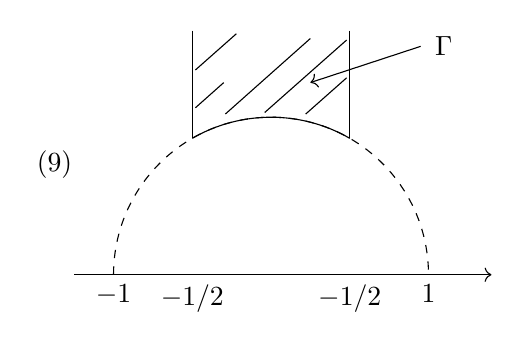
\begin{tikzpicture}[x=2cm,y=2cm]
\node[anchor=east] at (-1.2,.7) {(9)};
\draw[->] (-1.25,0)--(1.4,0);
\draw[dashed] (-1,0) arc[start angle=180,end angle=0,radius=1];
\draw (-.5,1.55)--(-.5,.866);
\draw (.5,1.55)--(.5,.866);
\draw (-.5,.866) arc[start angle=120,end angle=60,radius=1];
\draw (-.48,1.06)--(-.3,1.22);
\draw (-.48,1.3)--(-.22,1.53);
\draw (-.29,1.02)--(.25,1.5);
\draw (-.04,1.03)--(.48,1.49);
\draw (.22,1.02)--(.48,1.25);
\node[below] at (-1,0) {$-1$};
\node[below] at (-.5,0) {$-1/2$};
\node[below] at (.5,0) {$-1/2$};
\node[below] at (1,0) {$1$};
\draw[<-] (.25,1.22)--(.95,1.45);
\node[anchor=west] at (.98,1.45) {$\Gamma$};
\end{tikzpicture}
\end{adjustbox}
\end{center}
$\triangle$ с углами $\underbrace{0^{\circ},60^{\circ},60^{\circ}}$ на пл. Лобач.

Будем рассм. интегралы по $\triangle$-ку (9).

Выб. базис голом. квадр. дифф. на торе
\begin{equation*}
(10)\qquad f^1=1,\qquad \eta_1=\frac{1}{\operatorname{Im}\tau}
\end{equation*}
\begin{equation*}
d\Unclear{GELFAND-P001249}{du-overink}{u}
=dz+\delta y^1\frac{d\bar z}{\operatorname{Im}\tau}
\end{equation*}
[Перед объяснением $u$ зачёркнуто:]
\Incomplete{GELFAND-P001249}{u-cancel-full}{не удалось восстановить зачёркнутую запись перед новым комплексным обозначением}
$u$ — нов. компл. коорд. (компл. структура)

$y^1$ — новая коорд. в пр-ве модулей.
\begin{equation*}
(11)\qquad \text{Метр. содержит ровно 1 элемент:}\quad
\frac{dy^1\wedge d\bar y^1}{\operatorname{Im}\tau}
\end{equation*}

\SourcePage{GELFAND-P001250}{unlabelled}
\begin{equation*}
(12)\qquad \tau\longrightarrow\frac{u(\tau)}{u(1)}
=\frac{\tau+\delta y^1\bar\tau/\operatorname{Im}\tau}
{1+\delta y^1/\operatorname{Im}\tau}
\end{equation*}
\begin{equation*}
(13)\qquad u(z)=z+\delta y^1\frac{\bar z}{\operatorname{Im}\tau}
\end{equation*}
$y$ — координаты в пр-ве компл. структур

$y^1$ — любое, $\tau$ — вычисляется через $y^1$
\begin{equation*}
\frac{d\bar y^1\wedge dy^1}{\operatorname{Im}\tau}
=\frac{d\tau\wedge d\bar\tau}{4\operatorname{Im}\tau}
\end{equation*}
Теперь ост. вычислить:
\begin{equation*}
(14)\qquad \int_{\Gamma}\frac{d\tau\wedge d\bar\tau}{\operatorname{Im}\tau}
\frac{\int\mathcal D X_{\mu}\,e^{\int X_{\mu}\bar\partial\partial X^{\mu}\,dz\wedge d\bar z}}
{\int\mathcal D\varepsilon\,e^{\int\bar\varepsilon\bar\partial\partial\varepsilon\,dz\wedge d\bar z}}
\end{equation*}
[Под формулой, стрелка вверх к мере интегрирования:]
$\uparrow$ (Это не площадь! метрики).
И не удивит., т.к. начало не было инвар.

\begin{equation*}
(15)\qquad X_{\mu}=a_{\mu}^n X^n_{\ReaderApparatusRef{1}{2}},
\quad \Delta X^n_{\ReaderApparatusRef{2}{2}}
=\lambda^n X^n_{\ReaderApparatusRef{3}{2}}
\end{equation*}
Получим
\begin{equation*}
(16)\qquad
\frac{\int dX_{\mu}^0(\det'\Delta)^{-13}}
{\int d\varepsilon^0(\det'\Delta)^{-1}}
=\frac{V}{\operatorname{Im}\tau}(\det'\Delta)^{-12}
\end{equation*}
[Зачёркнуто: Ко\Incomplete{GELFAND-P001250}{cancel-word}{оставшаяся часть зачёркнутого слова перед Интегралы не читается}]
Интегралы по 0-й моде остаются;

вверху — объём вселенной (26-мерной)

внизу — площадь тора.

Положим $V=1$ временно.

Итог:
\begin{equation*}
(17)\qquad -\int_{\Gamma}
\frac{d\Unclear{GELFAND-P001250}{eq17-dtau}{\tau}\wedge d\bar\tau}
{(\operatorname{Im}\tau)^2}(\det'\Delta)^{-12}
\end{equation*}
[Внизу:] (из \Unclear{GELFAND-P001250}{bottom-abbrev}{ж.} пар-ии)
лишнее $\operatorname{Im}\tau$ $\Longrightarrow$ получилась площадь.


\ReaderNotesStart{GELFAND-P001250}
\ReaderNote{1}{\Incomplete{GELFAND-P001250}{eigen1-underink}{нечитаемый зачёркнутый нижний индекс}}
\ReaderNote{2}{\Incomplete{GELFAND-P001250}{eigen2-underink}{нечитаемый зачёркнутый нижний индекс}}
\ReaderNote{3}{\Incomplete{GELFAND-P001250}{eigen3-full}{нечитаемый зачёркнутый нижний индекс}}
\ReaderNotesEnd
\SourcePage{GELFAND-P001251}{59}
Как считать
\begin{equation*}
(18)\qquad (\det'\Delta)^{-1/2}
=\int\mathcal D\psi\,e^{-\int\partial\psi\bar\partial\psi\,dz\wedge d\bar z}
\end{equation*}
Будем считать вариацию его $\ln$ по вар. компл. структуры.

$\Delta$ обычный — по компл. структуре!
\begin{equation*}
(19)\qquad \delta\ln(\det'\Delta)^{-1/2}
\end{equation*}
Идея: базис, где диагонально и т.д.

\underline{Ответ:}
\begin{equation*}
(20)\qquad (\det'\Delta)^{-1/2}
=(\operatorname{Im}\tau)^{-1/2}e^{\frac{\pi}{6}\operatorname{Im}\tau}
\prod_{n=1}^{\infty}\lvert1-e^{2\pi in\tau}\rvert^{-2}
=(\operatorname{Im}\tau)^{-1/2}\lvert\eta(q)\rvert^{-2}
\end{equation*}
Для вычисления используем ф-лу (18)
\begin{equation*}
(21)\qquad \delta(\ln\det^{-1/2}\Delta)
=\frac{\delta\int\mathcal D\psi\,e^{-\int\partial\psi\bar\partial\psi\,d^2\xi}}
{\int\mathcal D\psi\,e^{-\int\partial\psi\bar\partial\psi\,d^2\xi}}
\end{equation*}
[После дроби зачёркнуто:]
\Incomplete{GELFAND-P001251}{fraction-tail-cancel}{не удалось прочитать зачёркнутую группу после дроби (21)}.

При этом:

[Перед вариацией зачёркнуто:]
\Incomplete{GELFAND-P001251}{metric-before-cancel}{не удалось разобрать зачёркнутую группу перед вариацией метрики}
\begin{equation*}
\delta(\sqrt g\,g^{ab}\partial_a\psi\partial_b\psi)=\delta g^{ab}T_{ab},
\end{equation*}
где
\begin{equation*}
T_{ab}=\partial_a\psi\partial_b\psi-\frac12g_{ab}
\partial^a_{\ReaderApparatusRef{1}{2}}\psi\partial^b\psi
\end{equation*}
\begin{equation*}
\delta g^{++}=\frac{\delta\tau}
{\ReaderApparatusRef{2}{2}\operatorname{Im}\tau},
\qquad \delta g^{--}=\frac{-\delta\bar\tau}
{\ReaderApparatusRef{3}{2}\operatorname{Im}\tau}
\qquad (?)
\end{equation*}
Итого
\begin{equation*}
(22)\qquad \delta(\ln\det^{-1/2}\Delta)
=2\operatorname{Re}\frac{i}{2}\delta\tau\langle T\rangle
\end{equation*}
(23) здесь $T$ — тензор энергии–импульса,
\begin{equation*}
T(\xi)=\frac{\int\mathcal D\psi\,\partial\psi(\xi)\partial\psi(\xi)
e^{-\int\partial\psi\bar\partial\psi\,d^2\xi}}
{\int\mathcal D\psi\,e^{-\int\partial\psi\bar\partial\psi\,d^2\xi}}
\end{equation*}
Общая ф-ла (на пов. $\forall$ рода)
\begin{equation*}
(24)\qquad \int d^2\xi\,(\eta T+\bar\eta\bar T).
\end{equation*}
[Справа, за двойной вертикальной чертой:]
$\partial\bar T=\bar\partial T_{+-}$.

($T$ — почти голом. дифференциал)

Более аккур. запись (23): надо заменить
$\partial\psi(\xi)\partial\psi(\xi)$ на $:\partial\psi(z)\partial\psi(z):$ и взять
\begin{equation*}
(25)\qquad T=:\partial\psi(z)\partial\psi(z):
\overset{\mathrm{def}}{=}\oint\frac{dz'}{2\pi i}\frac{1}{z'-z}
\partial\psi(z')\partial\psi(z)\quad\overset{\text{или}}{=}
\end{equation*}
\begin{equation*}
=\langle\partial\psi(z)\partial\psi(z)\rangle
\overset{\mathrm{def}}{=}\langle\oint\frac{dz'}{2\pi i}\frac{1}{z'-z}
\partial\psi(z')\partial\psi(z)
\end{equation*}


\ReaderNotesStart{GELFAND-P001251}
\ReaderNote{1}{\Incomplete{GELFAND-P001251}{stress-lower-cancel}{зачёркнутый нижний индекс под верхним a не читается}}
\ReaderNote{2}{\Incomplete{GELFAND-P001251}{gpp-cancel-full}{зачёркнутый префикс знаменателя перед Im не читается}}
\ReaderNote{3}{\Incomplete{GELFAND-P001251}{gmm-cancel-full}{зачёркнутый префикс знаменателя перед Im не читается}}
\ReaderNotesEnd
\SourcePage{GELFAND-P001252}{unlabelled}
Формула для любого рода.

Есть $p$ штук аб. дифф. $\omega_i$ и координаты
\begin{equation*}
(26)\qquad \vec z(Q)=\int_{Q_0}^{Q}\vec\omega
\end{equation*}
\begin{equation*}
(27)\qquad \int_{b_i}\omega_j=\tau_{ij},\qquad
\int_{a_i}\omega_j=\delta_i^j
\end{equation*}
Введ. ещё $\theta$-ф-и:
\begin{equation*}
\theta_{\bar\varepsilon,\delta}(\vec z\mid\hat\tau)
\ReaderApparatusRef{1}{2}
=\sum_{\vec n}e^{\pi i(n_i\hat\tau_{ik}n_k
\ReaderApparatusRef{2}{2}
+2\pi i\vec z\cdot(\vec n+\vec\delta)}
\end{equation*}
\begin{equation*}
\sum_{\vec n}e^{\pi i(\vec n+\vec\delta,\hat\tau,\vec n+\vec\delta)
+2\pi i(\vec z+\vec\varepsilon)(\vec n+\vec\delta)}
\end{equation*}
\begin{equation*}
4\vec\delta\cdot\vec\varepsilon\pmod 2
\end{equation*}
\begin{equation*}
\theta^*=\theta^{\bar\varepsilon,\bar\delta}_{,k}\omega_k(z);
\end{equation*}
[Стрелка к коэффициенту $\theta^{\bar\varepsilon,\bar\delta}_{,k}$:]
$\longleftarrow$ производная $\theta$ в нуле.

[Справа:] $\bar\varepsilon,\bar\delta$ — нечетная хар-ка.

из этого аб. дифф. можно извлечь корень (все нули — 2-го пор.).
\begin{equation*}
(28)\qquad T=\frac12
\underbrace{\left[\frac{\theta^{*''}}{\theta^*}
-\frac32\left(\frac{\theta^{*'}}{\theta^*}\right)^2\right]}_{\text{шварциан}}
-\frac16\frac{\theta_{ijk}\omega_i\omega_j\omega_k}{\theta'}
-\frac\pi2\omega_i(\operatorname{Im}\hat\tau)^{-1}_{ik}\omega_k
\end{equation*}
Всё это — вместе — квадратичный дифференциал.

$\omega$ не сод. $dz$: $\omega_i\,dz$ — форма.

\ReaderNotesStart{GELFAND-P001252}
\ReaderNote{1}{\Incomplete{GELFAND-P001252}{theta-arg-cancel}{неразборчивый зачёркнутый знак после первого аргумента theta}}
\ReaderNote{2}{\Incomplete{GELFAND-P001252}{theta-exp-r2}{неразборчивый зачёркнутый знак в первом показателе экспоненты}}
\ReaderNotesEnd

\end{document}
